%! Author = Omar Iskandarani
%! Title = Swirl-String Theory as an Emergent Relativistic Effective Field Theory with Preferred Foliation
%! Date = Aug 22, 2025
%! Affiliation = Independent Researcher, Groningen, The Netherlands
%! License = © 2025 Omar Iskandarani. All rights reserved. This manuscript is made available for academic reading and citation only. No republication, redistribution, or derivative works are permitted without explicit written permission from the author. Contact: info@omariskandarani.com
%! ORCID = 0009-0006-1686-3961
%! DOI = 10.5281/zenodo.16956665

\newcommand{\papertitle}{Swirl-String Theory as an Emergent Relativistic Effective Field Theory with Preferred Foliation}


\documentclass[smallextended]{svjour3}       % One-column layout
%\documentclass[twocolumn]{svjour3}          % Uncomment for two-column layout
\smartqed  % flush right qed marks
\usepackage{cite}
\usepackage{float}

%========================================================================================
% PACKAGES AND DOCUMENT CONFIGURATION
%========================================================================================

\usepackage{amsmath,amssymb,amsfonts}
\usepackage{graphicx}
\usepackage{microtype}
\usepackage{booktabs}
\usepackage{bookmark}
\usepackage{xcolor}
\usepackage{tcolorbox}
\usepackage{hyperref}
\usepackage{enumitem}
\usepackage{physics}
\usepackage{fancyhdr}

\usepackage{bm}

\usepackage{tikz}
\usetikzlibrary{knots,intersections,decorations.pathreplacing}
\usetikzlibrary{3d, calc, arrows.meta, positioning}
\usetikzlibrary{decorations.pathmorphing}

\usepackage{pgfmath}
\usepackage{pgfplots}
\pgfplotsset{compat=1.18} % or version you have

\usepackage{lmodern}
\usepackage{siunitx}
\sisetup{
    per-mode = symbol,
    exponent-product = \cdot,
    output-exponent-marker = \mathrm{e},
    detect-all,
}

\usepackage{mathtools}
\usepackage{ulem}
\usepackage[utf8]{inputenc}
\usepackage[T1]{fontenc}
\usepackage{longtable}
\usepackage[hyphens]{url}

% --- in preamble (optional but handy) ---
\newcommand{\cardwidth}{0.75\linewidth}
% ----------------------------------------


% Macro for hyperbolic volume (fixes undefined control sequence)
\newcommand{\VolH}[1]{\operatorname{Vol}_{\!\mathbb{H}}(#1)}

\newcommand{\swirlarrow}{%
	\mathchoice{\mkern-2mu\scriptstyle\boldsymbol{\circlearrowleft}}%
	{\mkern-2mu\scriptstyle\boldsymbol{\circlearrowleft}}%
	{\mkern-2mu\scriptscriptstyle\boldsymbol{\circlearrowleft}}%
	{\mkern-2mu\scriptscriptstyle\boldsymbol{\circlearrowleft}}%
}
\newcommand{\swirlarrowcw}{%
	\mathchoice{\mkern-2mu\scriptstyle\boldsymbol{\circlearrowright}}%
	{\mkern-2mu\scriptstyle\boldsymbol{\circlearrowright}}%
	{\mkern-2mu\scriptscriptstyle\boldsymbol{\circlearrowright}}%
	{\mkern-2mu\scriptscriptstyle\boldsymbol{\circlearrowright}}%
}
% --- Aliases to match legacy macro names used below ---
\newcommand{\Vol}{\operatorname{Vol}}   % now \Vol_{\!\mathbb{H}}(K) works
\newcommand{\rhof}{\rhoF}               % legacy \rhof -> current \rhoF

% Canonical symbols
\newcommand{\vswirl}{\mathbf{v}_{\swirlarrow}}
\newcommand{\vswirlcw}{\mathbf{v}_{\swirlarrowcw}}
\newcommand{\SwirlClock}{S_t^{\swirlarrow}}
\newcommand{\SwirlClockcw}{S_t^{\swirlarrowcw}}
\newcommand{\vnorm}{\lVert \vswirl \rVert} % generic speed magnitude
% --- local macros to avoid ambiguity ---
\providecommand{\rc}{r_c}
\providecommand{\vswirltext}{\mathbf{v}_{\mathrm{swirl}}} % textual variant if needed

% === House Notation Macros (mainstream field-theory style) ===
% Effective densities
\newcommand{\rhoF}{\rho_{\!f}}      % effective fluid density
\newcommand{\rhoE}{\rho_{\!E}}      % swirl energy density
\newcommand{\rhoM}{\rho_{\!m}}      % mass-equivalent density = \rhoE/c^2


\newcommand{\vstar}{v_\star}                           % canonical swirl-speed scale
% Tensor field strength (3-form) and 2-form potential
% (Already mainstream: H = dB, H_{mu nu rho} = \partial_{[mu} B_{nu rho]})
% Keep existing notation; define a convenience macro if desired:
\newcommand{\dB}{\,\mathrm{d}B} % optional use in forms notation
% === End Notation Macros ===

\newcommand{\xig}{\operatorname{asinh}\!\left(\tfrac{1}{2}\right)} % base hyperbolic scale
\newcommand{\phig}{\exp(\xig)} % golden from hyperbolic
\newcommand{\phialg}{\bigl(1+\sqrt{5}\bigr)/2} % algebraic echo (use sparingly)
\newcommand{\xigold}{\tfrac{3}{2}\,\xig} % "golden rapidity" scale

% --- Display helpers (optional) ---
\newcommand{\GoldenDeclare}{%
 \textbf{Golden (hyperbolic)}:\ \(\ln\phi=\xig\), hence \(\phi=\phig\).
 \ \emph{(Equivalently, \(\phi=\phialg\); this algebraic form is derivative.)}%
}

% --- Canonical identity (hyperbolic-only proof, algebraic as corollary) ---
\newtheorem{identity}{Identity}


%========================================================================================
% DOCUMENT START
%========================================================================================

\journalname{Foundations of Physics}

\begin{document}

\title{A Hydrodynamic Lagrangian Framework for Swirl--String Theory}

\author{Omar Iskandarani\thanks{ORCID: 0009-0006-1686-3961, DOI: 10.5281/zenodo.16956665}}
\institute{
    Omar Iskandarani \at
    Independent Researcher\\
    Groningen, The Netherlands\\
    \email{[info@omariskandarani.com]}
}

\date{Received: \today / Accepted: date}

\maketitle

\begin{abstract}
We present the Lagrangian formulation of Swirl–String Theory (SST), a fluid–topological effective field theory in which quantized circulation of an incompressible background generates matter and radiation. Closed knotted string excitations serve as particle states, and transverse swirl modes recover the Lorentz-invariant photon wave equation while dynamics unfold relative to an underlying foliation time. Mass follows from topological invariants via a canonical scaling law set by a single dimensionful constant, yielding parameter values that benchmark against observed lepton and baryon masses. The Lagrangian also accommodates parity-violating and contact terms, enabling interaction vertices analogous to Yukawa and weak couplings. The framework makes concrete predictions: I: quantized flux impulses from reconnection events, II: interference-visibility decay driven by finite-amplitude swirl, and III: skyrmionic photon textures indexed by knot chirality. SST thereby extends the tradition of hydrodynamic and analogue-gravity models while providing a testable, realist alternative to conventional quantum postulates.

\keywords{Swirl String Theory, Topological field theory, Quantum foundations, Vortex dynamics, Emergent spacetime}
\end{abstract}


%========================================================================================
%   INTRODUCTION
%========================================================================================
	\section{Introduction}

		The Standard Model and General Relativity capture a wide range of phenomena yet rest on disparate principles. An alternative—pursued from Kelvin’s swirl string atoms \cite{Kelvin1867}, through hydrodynamic formulations of quantum theory \cite{Madelung1927}, to modern topological solitons and analogue gravity \cite{Faddeev1997,Arnold1998,Barcelo2011,Volovik2003,Kleckner2013}—is that matter and interactions emerge from a structured, condensed vacuum. We develop an effective field theory (EFT) in which a preferred foliation, provided by a clock field \(T(x)\), endows the vacuum with order. In this medium, stable knotted swirl strings constitute the particle spectrum; their interactions arise from an emergent non-Abelian gauge structure built from coarse-grained vorticity.


		This framework, with its postulated swirl condensate and preferred foliation, can be formally classified as a modern Lorentz Ether Theory (LET). While empirically equivalent to Special Relativity in its kinematics, SST is not subject to the common Occam's Razor critique often applied to historical ether models. The swirl condensate is not an extraneous or undetectable component; it is the fundamental substrate whose topological and energetic properties are essential for deriving the particle mass spectrum from first principles—a predictive power with no direct equivalent in the Standard Model.

		Concretely, we introduce a unit timelike field \(u_\mu\) aligned with the foliation,
		\[
			u_\mu \equiv \frac{\partial_\mu T}{\sqrt{-g^{\alpha\beta}\partial_\alpha T\,\partial_\beta T}},
			\qquad u_\mu u^\mu = -1,
		\]
		and the spatial projector \(h_{\mu\nu}=g_{\mu\nu}+u_\mu u_\nu\) that selects dynamics on the leaves orthogonal to \(u_\mu\). A two-form \(B_{\mu\nu}\) with field strength \(H_{\mu\nu\rho}=\partial_{[\mu}B_{\nu\rho]}\) captures coherent vorticity of the condensed medium, while an emergent swirl connection \(\mathcal{W}_\mu\) with curvature \(\mathcal{W}_{\mu\nu}\) organizes interactions. A topological density \(\mathcal{W}_{\mu\nu}\tilde{\mathcal{W}}^{\mu\nu}\) enforces helicity quantization and stabilizes knotted configurations.

		Our central claim is operational: fermion rest masses arise as non-perturbative soliton energies of knotted swirl strings. We implement this via a calibrated mass functional fixed by condensate scales and knot invariants; at leading order we fit the constants on \((e^-,p,n)\) and predict the remaining masses \textbf{without introducing free Yukawa parameters}. Throughout we present the ontology and equations in a standard EFT form—covariant where possible and genuinely topological where stated—avoiding mixed nonrelativistic/relativistic constructs while making contact with analogue-gravity and topological-soliton frameworks through the \(H=dB\) sector and helicity-based stability.

%========================================================================================
%   FIELDS AND GEOMETRY
%========================================================================================
	\section{Foundational Fields and Geometry}
	\paragraph{Effective densities (mainstream field-theory style).}
	\begin{itemize}
		\item $\rhoF \equiv \text{effective fluid density}$
		\item $\rhoE \equiv \tfrac12\,\rhoF\,\vnorm^{2}\quad(\text{swirl energy density})$
        \item $\rhoM \;\equiv\; \frac{\rhoE}{c^2}\quad(\text{mass-equivalent density})$
	\end{itemize}


	We work on a 4D Lorentzian manifold with metric \(g_{\mu\nu}\) of signature \((-+++)\). The totally antisymmetric tensor satisfies \(\varepsilon^{0123}=+1\); antisymmetrization is \(X_{[\mu\nu]}=\tfrac12(X_{\mu\nu}-X_{\nu\mu})\). Indices are raised/lowered with \(g_{\mu\nu}\).

	\begin{itemize}
		\item \textbf{Clock Field \(T(x)\) and Preferred Foliation.}
		Define the unit timelike condensate 4-velocity
		\begin{equation}
			u_{\mu} \equiv \frac{\partial_{\mu}T}{\sqrt{-\,\partial_{\alpha}T\, \partial^{\alpha}T}},
			\qquad u_\mu u^\mu=-1,
		\end{equation}
		which is invariant under monotone reparametrizations \(T\!\to\! f(T)\).
		The spatial projector onto leaves orthogonal to \(u_\mu\) is
		\begin{equation}
			h_{\mu\nu} \equiv g_{\mu\nu}+u_\mu u_\nu, \qquad h_{\mu\nu}u^\nu=0, \qquad h^\mu{}_\alpha h^\alpha{}_\nu=h^\mu{}_\nu.
		\end{equation}
		Integrability of the foliation is equivalent to the Frobenius condition \(u_{[\mu}\nabla_{\nu}u_{\rho]}=0\), which holds when \(u_\mu\propto\partial_\mu T\).

		\item \textbf{Condensate Modulus \(\Phi\).}
		A real scalar controlling medium scales (stiffness, characteristic speeds). We write \(\Phi(x)=\Phi_0+\delta\Phi(x)\) about a homogeneous vacuum value \(\Phi_0>0\). This \emph{is not} the Standard Model Higgs; it does not introduce Yukawa parameters.

		\item \textbf{Two-Form Potential \(B_{\mu\nu}\) and Three-Form Field Strength \(H\).}
		\begin{equation}
			H_{\mu\nu\rho} \equiv \partial_{[\mu} B_{\nu\rho]} \quad (\;= \tfrac{1}{3!}\,\varepsilon_{\mu\nu\rho\sigma}\,\tilde H^{\sigma}\;).
		\end{equation}
		Gauge symmetry: \(B \mapsto B + d\Lambda\) with 1-form \(\Lambda_\mu\). Bianchi identity: \(\partial_{[\sigma}H_{\mu\nu\rho]}=0\).
		Swirl strings couple electrically to \(B\) (worldsheet term \(\int_\Sigma B\)); their topological charge is measured by fluxes of \(H\).

		\item \textbf{Emergent Swirl Connection \(\mathcal{W}_\mu^a\).}
		A non-Abelian gauge potential for coarse-grained vorticity modes valued in a compact Lie algebra with structure constants \(f^{abc}\).
		\begin{equation}
			\mathcal{W}_{\mu\nu}^a \equiv \partial_\mu \mathcal{W}_\nu^a - \partial_\nu \mathcal{W}_\mu^a + g_{\!sw}\, f^{abc}\,\mathcal{W}_\mu^b \mathcal{W}_\nu^c,
			\qquad \tilde{\mathcal{W}}^{\mu\nu a} \equiv \tfrac12 \varepsilon^{\mu\nu\rho\sigma}\mathcal{W}_{\rho\sigma}^a .
		\end{equation}
		Gauge transformations act as \(\delta \mathcal{W}_\mu^a = -(\nabla_\mu \alpha)^a - g_{\!sw} f^{abc}\alpha^b \mathcal{W}_\mu^c\),
		and on matter via the covariant derivative \(D_\mu=\nabla_\mu + g_{\!sw}\,\mathcal{W}_\mu^a T^a\) with generators \(T^a\).

		\item \textbf{Knot Fermion Fields \(\Psi_K\).}
		Effective relativistic spinors associated with stable knotted swirl strings labeled by topological class \(K\) (e.g., torus knots). Their rest masses are non-perturbative soliton energies \(m_K^{(\mathrm{sol})}\). They transform under the swirl gauge group via \(D_\mu\Psi_K\).

	\end{itemize}

	\paragraph{Dimensional assignments (natural units \(\hbar=c=1\)).}
	\([ \mathcal{W}_\mu ]=1,\; [ \mathcal{W}_{\mu\nu} ]=2,\; [ B_{\mu\nu} ]=1,\; [ H_{\mu\nu\rho} ]=2,\; [ \Phi ]=1,\; [ \Psi ]=\tfrac{3}{2},\; [g_{\!sw}]=0.\)

% --- Integrated: Clock Foliation Dynamics and Constraints ---
	\subsection{Clock Foliation Dynamics and Constraints}
	Define the unit timelike foliation vector by
	\begin{equation}
		u_\mu \equiv \frac{\partial_\mu T}{\sqrt{-g^{\alpha\beta}\partial_\alpha T\partial_\beta T}},\qquad u_\mu u^\mu=-1.
	\end{equation}
	We include the foliation-unit (khronon) sector
	\begin{align}
		\mathcal L_{T} \;=\; \frac{M_u^{2}}{2}\Big[&c_1(\nabla_\mu u_\nu)(\nabla^\mu u^\nu)+c_2(\nabla_\mu u^\mu)^2+c_3(\nabla_\mu u_\nu)(\nabla^\nu u^\mu)\\
		&+c_4\,u^\mu u^\nu (\nabla_\mu u_\alpha)(\nabla_\nu u^\alpha)\Big]
		\;+\;\lambda\,(u_\mu u^\mu+1).\nonumber
	\end{align}
	This sector is invariant under monotone reparametrizations \(T\mapsto f(T)\), and since \(u\propto\nabla T\) the foliation is integrable (Frobenius).

	A cosmological origin follows from a shift--symmetric condensate \(T(x)=\mu t+\pi(x)\) with timelike gradient \(X=g^{\mu\nu}\partial_\mu T\partial_\nu T<0\) and
	\(\mathcal L_{\textrm khr}(X)=M_\star^4\,P(X/M_\star^4)\). In unitary gauge this reproduces \(\mathcal L_T\).

	\paragraph{Observational constraints.}
	The tensor-mode speed is
	\(c_T^2=\frac{1}{1-c_{13}}\) with \(c_{13}=c_1+c_3\). The binary neutron-star event GW170817/GRB170817A implies \(|c_T/c-1|\lesssim10^{-15}\), so we take the baseline fit \(c_{13}=0\).
	Preferred-frame PPN parameters \(\alpha_1(c_i),\alpha_2(c_i)\) constrain the remaining combinations, and the absence of gravitational \v{C}erenkov losses requires \(c_T\ge 1\).
	Non-gravitational LIV constraints can be tracked via the SME Data Tables.


	\begin{table}[h]
		\centering
		\caption{Clock-sector parameters and baseline constraint.}
        \resizebox{\textwidth}{!}{%
		\begin{tabular}{lcc}
			\hline
			Parameter & Meaning & Baseline / Constraint \\
			\hline
			$c_{13} \equiv c_1 + c_3$ & controls tensor speed $c_T^2=\frac{1}{1-c_{13}}$ & set to $0$ (GW170817) \\
			$c_1,c_2,c_4$ & foliation-vector couplings in $\mathcal{L}_T$ & to be bounded in scans \\
			$M_u$ & foliation sector scale & free EFT scale \\
			\hline
		\end{tabular}
        }
	\end{table}

	\paragraph{Coarse--graining between leaf rotation and fluid density.}
	\begin{equation}
		K \equiv \frac{\rhoM\, r_c}{\vswirl},
		\qquad
		\rhoF \;=\; K\,\Omega .
	\end{equation}
	With Canon constants: \(K = 5.01509060\times 10^{-3}\ \mathrm{kg\,m^{-3}\,s}\), \(\Omega^\ast = 1.39578735\times 10^{-4}\ \mathrm{s^{-1}}\), and \(T^\ast=2\pi/\Omega^\ast\approx 12.50\ \mathrm{h}\).
% --- End Integrated block ---


%========================================================================================
%   EFFECTIVE ACTION (CONSISTENT, COVARIANT)
%========================================================================================
	\section{Effective Action}

	A minimal, consistent Lagrangian density implementing the ingredients above is

    \begin{align}
    \mathcal{L}
    =&-\frac{\kappa_\omega}{4}\,\mathcal{W}^a_{\mu\nu}\,\mathcal{W}^{a\mu\nu}
    +\frac{\kappa_B}{12}\,H_{\mu\nu\rho}\,H^{\mu\nu\rho}
    +\frac{1}{2}(\nabla_\mu\Phi)(\nabla^\mu\Phi)
    -V(\Phi) \nonumber\\
    &\quad
    +\frac{\theta}{4}\,\mathcal{W}^a_{\mu\nu}\,\tilde{\mathcal{W}}^{a\mu\nu}
    +\lambda_1\,(u_\mu u^\mu+1)
    +\lambda_2\,\nabla_\mu u^\mu \nonumber\\
    &\quad
    +\sum_K \bar\Psi_K\!\left(i\gamma^\mu D_\mu - m_K^{(\mathrm{sol})}\right)\!\Psi_K \,,
    \label{eq:EFT}
    \end{align}


	with
	\[
		H_{\mu\nu\rho}\equiv \partial_{[\mu}B_{\nu\rho]},\qquad
		\tilde{\mathcal{W}}^{a\mu\nu}\equiv \tfrac{1}{2}\,\varepsilon^{\mu\nu\rho\sigma}\,\mathcal{W}^a_{\rho\sigma},\qquad
		D_\mu\equiv \nabla_\mu + i g_{\!sw}\,\mathcal{W}_\mu^a T^a .
	\]
	We adopt \(\varepsilon^{0123}=+1\) and the \((-+++)\) metric signature.
	Here \(\nabla_\mu\) is the Levi–Civita (spin-)covariant derivative; on spinors it includes the spin connection.

	\paragraph{Symmetries and constraints.}
	The theory is invariant under
	\(B\mapsto B+d\Lambda\) (2-form gauge) and local swirl-gauge transformations
	\(\mathcal{W}_\mu \mapsto U^{-1}\!\big(\mathcal{W}_\mu + \tfrac{i}{g_{\!sw}}\partial_\mu\big)U\),
	\(\Psi_K\mapsto U^{-1}\Psi_K\).
	The Lagrange multipliers enforce a unit timelike condensate velocity and, if desired, covariant incompressibility \(\nabla_\mu u^\mu=0\).
	The \(\theta\)-term \(\mathcal{W}\tilde{\mathcal{W}}\) is the non-Abelian Chern–Pontryagin density (a total derivative); in the present context it encodes helicity/knot-charge conservation.

	\paragraph{Spinor fields as emergent quasiparticles.}
	The Dirac term in \eqref{eq:EFT} provides the low-energy description of stabilized knotted swirl excitations labeled by a topological class \(K\) (e.g., torus knots). Their rest masses \(m_K^{(\mathrm{sol})}\) are non-perturbative soliton energies determined by the calibrated mass functional introduced later. The spinors transform under the swirl gauge group \(G_{\!sw}\) via \(D_\mu\).

	\paragraph{Remarks.}
	(I) No fundamental Yukawa couplings are introduced; fermion masses enter only through soliton energies.
	(II) Any gauge-boson screening/mass arises from medium effects (e.g., \(\Phi\)-dependent polarization) rather than SM-style Higgs couplings.
	(III) Appendix~\ref{sec:swirl-connection} outlines the coarse-grained origin of the swirl connection \(\mathcal{W}_\mu^a\).

    \begin{figure}[h!]
    \centering
    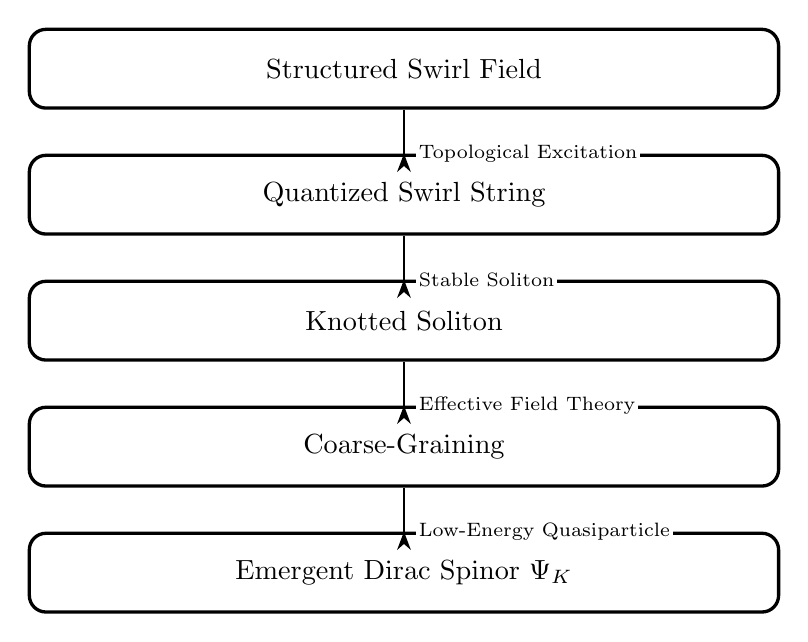
\begin{tikzpicture}[
        y=1.6cm, x=1cm,
        box/.style={
            rectangle, draw=black, very thick, rounded corners=6pt, fill=white,
            minimum height=10mm, text width=\cardwidth, align=center, inner sep=6pt
        },
        arrow/.style={-Stealth, thick},
        lab/.style={font=\scriptsize, fill=white, inner sep=1pt}
    ]
        % Nodes (top to bottom)
    \node[box] (condensate) at (0,0)   {Structured Swirl Field};
    \node[box] (string)     at (0,-1)  {Quantized Swirl String};
    \node[box] (knot)       at (0,-2)  {Knotted Soliton};
    \node[box] (coarse)     at (0,-3)  {Coarse-Graining};
    \node[box] (dirac)      at (0,-4)  {Emergent Dirac Spinor $\Psi_K$};

    % Short vertical arrows with labels on the right
    \draw[arrow] (condensate.south) -- ++(0,-0.35) node[lab, right=4pt] {Topological Excitation} |- (string.north);
    \draw[arrow] (string.south) -- ++(0,-0.35) node[lab, right=4pt] {Stable Soliton} |- (knot.north);
    \draw[arrow] (knot.south) -- ++(0,-0.35) node[lab, right=4pt] {Effective Field Theory} |- (coarse.north);
    \draw[arrow] (coarse.south) -- ++(0,-0.35) node[lab, right=4pt] {Low-Energy Quasiparticle} |- (dirac.north);
    \end{tikzpicture}
    \caption{Emergence of effective spinor fields in Swirl–String Theory.}
    \label{fig:emergent-spinors-vertical}
    \end{figure}



%========================================================================================
%   EMERGENT MASS FROM SOLITON ENERGY
%========================================================================================
	\section{Emergent Mass from Soliton Energy}
	\label{sec:mass-functional}
	For a static, stable knotted swirl configuration \(K\), the rest energy \(E_K\) defines the solitonic mass.
	Working in natural units \(\hbar=c=1\),
	\begin{equation}
		m_K^{(\mathrm{sol})} = E_K .
	\end{equation}

	Guided by semiclassical analyses of knotted solitons \cite{Faddeev1997} and swirl energetics, we employ a \emph{topological mass functional}
	\begin{equation}
		\boxed{ \; m_K^{(\mathrm{sol})} = \mathcal{M}_0 \,\Xi_K(m,n,s,k;\,\varphi) \; }
		\label{eq:mass-functional}
	\end{equation}
	where \(\mathcal{M}_0\) sets a universal energy scale and \(\Xi_K\) is a dimensionless topological factor.

	We implement this via a calibrated functional fixed by condensate scales and knot invariants. At leading order we fit the constants on \((e^{-},p,n)\) and predict the remaining masses \emph{without introducing free Yukawa parameters} (see Appendix~\ref{sec:knot-particle-mapping} for the calibration hierarchy and the lepton analysis).

	\paragraph{Core scale.}
	Introduce the \emph{core swirl speed scale} \(\vstar\) (Appendix~\ref{sec:calibration-hierarchy}). We take
	\begin{equation}
		\boxed{ \; \mathcal{M}_0 \equiv C_0 \left(\sum_i V_i\right)\,\rhoF\,\vstar^{\,2} \; }
		\label{eq:M0}
	\end{equation}
	with
	(I) \( \sum_i V_i \): total effective core volume of the knot (tube model),
	(II) \( \rhoF \): base energy density of the medium (Appendix~\ref{sec:calibration_rho0}),
	(III) \(C_0\): dimensionless normalization capturing geometric/logarithmic slenderness and finite-core effects.

	\paragraph{Topological factor.}
	\(\Xi_K\) encodes geometric/dynamical properties of the knot:
    \[
        \Xi_K = \Xi_K(m,n,s,k;\,\varphi),\qquad
        \begin{aligned}
        m&=\text{strand multiplicity},\; n=\text{knot/link index},\\
        s&=\text{coherence/tension index},\; k=\text{layer index}.
        \end{aligned}
    \]

	A concrete ansatz used below is
	\begin{equation}
		\Xi_K(m,n,s,k;\,\varphi) = \frac{\mathcal{T}_K(m,n,s)}{\varphi^{\,2k}},
		\label{eq:Xi-ansatz}
	\end{equation}
	where \(\mathcal{T}_K\) is a dimensionless tangle measure (e.g., normalized ropelength or writhe), and \(\varphi\) enters through canonical core geometry (Sec.~\ref{sec:golden_layer}).

	\subsection{Heuristic derivation of the mass functional}

	\paragraph{(1) Core energy from swirl-string dynamics.}
	For an incompressible medium, the energy per unit length of a slender swirl string scales as
	\(
	\tfrac{dE}{d\ell} \sim \tfrac{1}{2}\rhoF\,\Gamma^2 \ln (R/\rc)
	\).
	With \(\Gamma \sim \vstar\,\rc\) and total arclength \(\ell_K\),
	\begin{equation}
		E_K^{\mathrm{core}} \sim \rhoF\,\vstar^{\,2}\,\ell_K \ln\!\left(\frac{R}{\rc}\right).
	\end{equation}

	\paragraph{(2) Volume correction (tube model).}
	Treat each strand as a tube of radius \(\rc\):
	\(
	V_K=\sum_i \pi \rc^2 \ell_i
	\Rightarrow
	E_K^{\mathrm{bulk}} \sim \rhoF\,\vstar^{\,2}\,V_K
	\),
	which dominates for compact, tightly wound knots.
	See Appendix~\ref{sec:knot-particle-mapping} for the explicit knot\(\to\)particle dictionary.

	\paragraph{(3) Topological suppression via coherence.}
	To encode knot geometry and internal alignment, introduce \(\Xi_K\) as in \eqref{eq:Xi-ansatz}. The factor \(\varphi^{-2k}\) models discrete coherence layers within the core (Sec.~\ref{sec:golden_layer}), while \(\mathcal{T}_K\) captures shape-dependent tangle energy.

	\paragraph{(4) Combined result.}
	Collecting pieces yields \eqref{eq:mass-functional} with \(\mathcal{M}_0\) as in \eqref{eq:M0}.

	\paragraph{Dimensional check.}
	In \(\hbar=c=1\), \([\rhoF]=4\), \([V]=(-3)\), \([\vstar]=0\) \(\Rightarrow\) \([\mathcal{M}_0]=1\) (mass), as required. \(\Xi_K\) is dimensionless by construction.

	\subsection{Calibration and comparison}

	Fix \(\mathcal{M}_0\) on a single reference (electron) to set the overall scale:
	\begin{equation}
		C_0
		= \frac{m_e}{\big(\sum_i V_i\big)_e \,\rhoF \,\vstar^{\,2}}\,
		\frac{1}{\Xi_{K_e}} .
		\label{eq:calibration}
	\end{equation}
	After \eqref{eq:calibration}, predictions are parameter-free:
	\[
		\frac{m_K^{(\mathrm{sol})}}{m_{K'}^{(\mathrm{sol})}}
		\;=\; \frac{\Xi_K}{\Xi_{K'}}.
	\]
	Uncertainties propagate via
	\begin{equation}
		\delta m_K^2 \simeq m_K^2\Big[
			\big(\delta\rhoF/\rhoF\big)^2
			+ \big(2\,\delta\vstar/\vstar\big)^2
			+ \big(\delta V/V\big)^2
			+ \big(\delta\Xi_K/\Xi_K\big)^2
			\Big].
	\end{equation}
	Comparisons use experimental values \cite{PDG2024}; medium/self-interaction corrections can be layered as perturbations to \(\rhoF\) or to \(\mathcal{T}_K\).

%===========================================================
	\subsection{Golden Layer: Hyperbolic Canonical Definition}
	\label{sec:golden_layer}
%===========================================================

	\paragraph*{Policy (hyperbolic-first).}
	Define the golden constant hyperbolically:
	\[
		\xi_\varphi \;\equiv\; \operatorname{asinh}\!\left(\tfrac{1}{2}\right),
		\qquad
		\varphi \;\equiv\; \exp(\xi_\varphi),
	\]
	and note the algebraic echo \(\varphi=(1+\sqrt5)/2\) only as a corollary.

	\paragraph*{Golden rapidity.}
	Let
	\[
		\xi_g \;\equiv\; \tfrac{3}{2}\,\xi_\varphi.
	\]
	Using \(\tanh y=\dfrac{e^{2y}-1}{e^{2y}+1}\) \cite{NISTDLMF} and \(\varphi=\exp(\xi_\varphi)\) with \(\varphi^2=\varphi+1\),
	\[
		\tanh(\xi_g) \;=\; \frac{\varphi^3-1}{\varphi^3+1}
		\;=\; \frac{1}{\varphi}.
	\]
	Therefore
	\[
		\boxed{\ \tanh\!\big(\tfrac{3}{2}\,\xi_\varphi\big)=\tanh(\xi_g)=\varphi^{-1}\ },
		\qquad\text{equivalently}\ \ \coth(\xi_g)=\varphi.
	\]

	\paragraph*{SST mapping (canonical scales).}
	Let \(v\equiv\|\vswirl\|\). Parametrize swirl speed by rapidity via
	\[
		\beta \;\equiv\; \frac{v}{\vstar} \;=\; \tanh\xi;
	\]
	at the Golden Layer \(\xi=\xi_g\),
	\[
		\beta_g \;=\; \frac{1}{\varphi},\qquad
		v_g \;=\; \beta_g\,\vstar \;=\; \frac{\vstar}{\varphi},\qquad
		\Omega_g \;=\; \frac{v_g}{\rc} \;=\; \frac{1}{\varphi}\,\frac{\vstar}{\rc}.
	\]
	\emph{Dimensional check:} \([\beta_g]=1\), \([v_g]=\mathrm{m/s}\), \([\Omega_g]=\mathrm{s}^{-1}\).

	\paragraph*{Algebraic echo (post-hoc).}
	From \(\operatorname{asinh}x=\ln(x+\sqrt{x^2+1})\) \cite{NISTDLMF},
	\[
		\xi_\varphi=\operatorname{asinh}\!\left(\tfrac{1}{2}\right)
		=\ln\!\left(\tfrac{1}{2}+\sqrt{\tfrac{1}{4}+1}\right)
		=\ln\!\left(\tfrac{1+\sqrt5}{2}\right),
	\]
	so \(\varphi=\exp(\xi_\varphi)=(1+\sqrt5)/2\).

	\paragraph*{Numerical evaluation (Canon constants).}
	With \(\vstar=\SI{1.09384563e6}{m/s}\) and \(\rc=\SI{1.40897017e-15}{m}\),
	\[
		\varphi \approx 1.618033988749895,\quad
		\xi_g=\tfrac{3}{2}\ln\varphi \approx 0.721817737589405,
	\]
	\[
		\beta_g=\tanh\xi_g=\varphi^{-1}\approx 0.618033988749895,\qquad
		v_g=\frac{\vstar}{\varphi}\approx \SI{6.760337778e5}{m/s},
	\]
	\[
		\Omega_{\!*}=\frac{\vstar}{\rc}\approx \SI{7.763440655e20}{s^{-1}},\qquad
		\Omega_g=\frac{\Omega_{\!*}}{\varphi}\approx \SI{4.798070195e20}{s^{-1}}.
	\]

	\paragraph*{On the \(3/2\) exponent.}
	The factor \(\tfrac{3}{2}\) in \(\xi_g\) mirrors familiar spectral/dispersion scalings (e.g., level spacings, Kelvin-wave cascades) and labels “golden layers” in SST.

	\subsection{Pentagonal resonance hypothesis}
	\paragraph*{Remark (pentagon transient).}
	When an unknotting filament strikes a boundary, a short-lived five-vertex symmetry (pentagon-like) is empirically observed; in SST this is treated as a \emph{transient morphometric feature} of curvature–torsion flow rather than a defining identity for \(\varphi\). Motivated by simulations of swirl string–ring impacts \cite{orlandi1993vortex}, we hypothesize:
	\begin{quote}
		\textbf{Pentagonal Resonance Hypothesis.}
		A photon is absorbed by an electron when its transient pentagonal swirl mode geometrically resonates with a pentagonal face of the dodecahedral electron shell, enabling energy and swirl transfer.
	\end{quote}

	\subsection{Canonical role}
	The Golden Layer functions as (I) a \emph{quantization anchor} for swirl rapidity (\(\xi=\xi_g\)); (II) a \emph{resonance mechanism} in electron–photon coupling via dodecahedral symmetry; and (III) a \emph{bridge} between continuous swirl dynamics and discrete spectroscopic structure.

% --- Integrated: EFT derivation of alpha_C C + beta_L L and golden-layer ---
	\subsection{Field-Theoretic Derivation of \texorpdfstring{$\alpha_C C+\beta_{\!L} L$}{alpha_C C + beta_L L} and \texorpdfstring{$\varphi^{-2k}$}{phi^{-2k}}}
	\paragraph*{Length term.}
	For a slender tube of radius \(\rc\) and circulation \(\Gamma\), the line tension is
	\(
	\tau\simeq \frac{\rhoF\Gamma^2}{4\pi}\ln\!\frac{R}{\rc}+\kappa_H \rc^2\langle\omega^2\rangle
	\),
	so \(E_{\textrm line}\simeq \tau\,\ell_K\),
	and with \(L(K)=\ell_K/\rc\) this yields a contribution \(\propto \beta_{\!L}\,L(K)\).

	\paragraph*{Crossing term.}
	Nonlocal Biot--Savart interactions between tube segments near contact (\(\sim \rc\)) discretize to counts proportional to the minimal crossing number \(C(K)\), giving
	the term \(\propto \alpha_C\,C(K)\). A Skyrme/Hopf quartic term enforces the stability bound \(E\ge \kappa\,|Q_H|^{3/4}\).

	\paragraph*{Golden-layer suppression.}
	A weak pentagonal core deformation induces discrete scale invariance in radial modes with ratio \(\lambda_\star=\varphi\).
	Since energy scales with amplitude squared, this yields the multiplicative factor \(\varphi^{-2k}\) for the \(k\)-th layer.
	Altogether (with your normalization),
	\begin{equation}
		\Xi_K \;=\; \frac{\alpha_C\,C(K)+\beta_{\!L}\,L(K)}{T_{01}}\;\varphi^{-2k_K},
		\qquad
		m_K \;=\; \mathcal{M}_0\,\Xi_K .
	\end{equation}


%========================================================================================
%   GAUGE STRUCTURE AND CHARGES
%========================================================================================
	\section{Gauge Structure and Charge Assignment}

	\paragraph{Emergent swirl gauge group.}
	The mesoscale vorticity modes organize into an emergent non-Abelian group \(G_{\!sw}\) with generators \(T^a\) and connection \(\mathcal{W}_\mu=\mathcal{W}_\mu^a T^a\).
	Matter fields \(\Psi_K\) (knotted excitations) couple via \(D_\mu=\nabla_\mu+i g_{\!sw}\,\mathcal{W}_\mu\).
	The Chern–Pontryagin density \(\mathcal{W}_{\mu\nu}^a\tilde{\mathcal{W}}^{a\mu\nu}\) tracks conserved knot/helicity charge in the swirl sector.

	\paragraph{Low-energy image and charge map.}
	At low energies we use a homomorphism
	\[
		\pi:\; G_{\!sw}\longrightarrow G_{\textrm SM}\equiv SU(3)_c\times SU(2)_L\times U(1)_Y,
	\]
	fixed by knot invariants of \(K\).
	Let the minimal topological data be
	\[
		\mathbf{t}(K)\equiv\big(L_K\!\!\!\!\pmod{3},\; S_K\!\!\!\!\pmod{2},\; \chi_K\big),
	\]
	where \(L_K\in\mathbb{Z}\) is a net linking index (with an ambient color flux), \(S_K\in\mathbb{Z}\) is a self-linking parity (writhe+twist), and \(\chi_K\in\{+1,-1\}\) is the knot chirality (orientation).
	We assign:
	\begin{align}
		&\text{color rep:} &&
		R_c(K)=
		\begin{cases}
			\mathbf{1} & \text{if } L_K\equiv 0\ (\mathrm{mod}\ 3),\\
			\mathbf{3} & \text{if } L_K\equiv 1,2\ (\mathrm{mod}\ 3),
		\end{cases}
		\\[2pt]
		&\text{weak rep:} &&
		R_L(K)=
		\begin{cases}
			\mathbf{2} & \text{if } S_K\equiv 1\ (\mathrm{mod}\ 2),\\
			\mathbf{1} & \text{if } S_K\equiv 0\ (\mathrm{mod}\ 2),
		\end{cases}
		\\[2pt]
		&\text{weak isospin:} &&
		T_3(K)=
		\begin{cases}
			+\tfrac{1}{2} & \text{if } R_L=\mathbf{2}\ \text{and }\chi_K=+1,\\
			-\tfrac{1}{2} & \text{if } R_L=\mathbf{2}\ \text{and }\chi_K=-1,\\
			0 & \text{if } R_L=\mathbf{1},
		\end{cases}
		\\[2pt]
		&\text{hypercharge:} &&
		Y(K)=\alpha\,S_K+\beta\,\chi_K+\gamma\,\delta_{R_c,\mathbf{3}}+\delta,
		\label{eq:Y-map}
	\end{align}
	with integer-quantized coefficients \(\alpha,\beta,\gamma, \delta\) fixed once and for all by matching a single generation’s observed charges; see Appendix~\ref{sec:knot-particle-mapping}.
	Electric charge follows \(Q=T_3+\tfrac12 Y\).

    % Insert this snippet into Section V (Gauge Structure and Charge Assignment),
% immediately after equation (20) and the one-generation worked check.

\subsection*{Complete Mapping of the Twelve SM Fermions to Knotted Swirl-String States}

For clarity and falsifiability, we collect here a complete assignment of the twelve Standard Model (SM) fermions to specific knotted/linked swirl-string configurations~\ref{tab:SM12_knot_map}. The mapping respects the SST taxonomy (charged leptons \,$\leftrightarrow$\, torus knots; neutrinos \,$\leftrightarrow$\, linked states; quarks \,$\leftrightarrow$\, chiral hyperbolic knots), the invariant triple
\(t(K) = \big(L_K \bmod 3,\, S_K \bmod 2,\, \chi_K\big)\), and the charge map of Eq.~(20). Color is fixed by \(L_K\): leptons have \(L_K\equiv 0\) (color singlets), quarks have \(L_K\equiv 1,2\) (color triplets). Left-handed (LH) fermions sit in weak doublets via \(S_K=1\) and acquire \(T_3=\pm\tfrac12\) with the sign set by \(\chi_K=\pm 1\); right-handed (RH) partners are weak singlets with \(S_K=0\) and \(T_3=0\). Once the linear coefficients \((\alpha,\beta,\gamma,\delta)\) in Eq.~(20) are fixed on a single generation, the electric charges \(Q = T_3 + \tfrac12 Y\) follow for all flavors. We retain the canonical anchors \(u\leftrightarrow 5_2\) and \(d\leftrightarrow 6_1\).

    \begin{table}[htbp]
        \caption{\textbf{Mapping of the 12 Standard Model Fermions to Swirl String Theory (SST) Knotted States, with Predicted Electric Charge.}}
        \centering
        \renewcommand{\arraystretch}{1.15}
        \setlength{\tabcolsep}{0.45em}
        \resizebox{\textwidth}{!}{%
            \begin{tabular}{lccccccc}
                \toprule
                \textbf{SM Fermion} & \textbf{SST Knot/Link} & \textbf{Periods} & \textbf{Chiral?} & \textbf{FSG} & \textbf{Knot Type} & \textbf{$t(K)=(L,S,\chi)$} & \textbf{$Q$}\\
                &  &  &  &  &  & \textbf{(LH / RH)} &  \\
                \midrule
                $e^-$ (electron) & $3_1$ (trefoil, $T(2,3)$) & $2,3$ & Yes & $Z_2$ & Torus knot & $(0,1,-1)$ / $(0,0,\cdot)$ & $-1$ \\
                $\mu^-$ (muon)   & $5_1$ (cinquefoil, $T(2,5)$) & $2,5$ & Yes & $Z_2$ & Torus knot & $(0,1,-1)$ / $(0,0,\cdot)$ & $-1$ \\
                $\tau^-$ (tau)   & $7_1$ (septfoil, $T(2,7)$) & $2,7$ & Yes & $Z_2$ & Torus knot & $(0,1,-1)$ / $(0,0,\cdot)$ & $-1$ \\
                \midrule
                $\nu_e$          & Hopf link $2^2_1$ & $2$ & No & $D_4$ & 2-comp link & $(0,1,+1)$ / $(0,0,\cdot)$ & $0$ \\
                $\nu_\mu$        & $12a_{1202}$ & $2,6$ & No & $D_{12}$ & 2-comp link & $(0,1,+1)$ / $(0,0,\cdot)$ & $0$ \\
                $\nu_\tau$       & amphichiral 2-comp link (6--8 cr.) & $2,4$ & No & $D_8$ & 2-comp link & $(0,1,+1)$ / $(0,0,\cdot)$ & $0$ \\
                \midrule
                $u$ (up)         & $5_2$ \textit{(canonical)} & $2$ & Yes & $D_4$ & Hyperbolic knot & $(1,1,+1)$ / $(1,0,\cdot)$ & $\tfrac{2}{3}$ \\
                $c$ (charm)      & $8_{19}$ & $2,3,4$ & Yes & $Z_2$ & Hyperbolic knot & $(1,1,+1)$ / $(1,0,\cdot)$ & $\tfrac{2}{3}$ \\
                $t$ (top)        & $8_{21}$ & $2$ & Yes & $D_4$ & Hyperbolic knot & $(1,1,+1)$ / $(1,0,\cdot)$ & $\tfrac{2}{3}$ \\
                \midrule
                $d$ (down)       & $6_1$ \textit{(canonical)} & $2$ & Yes & $D_8$ & Hyperbolic knot & $(2,1,-1)$ / $(2,0,\cdot)$ & $-\tfrac{1}{3}$ \\
                $s$ (strange)    & $7_5$ & $2$ & Yes & $D_4$ & Hyperbolic knot & $(2,1,-1)$ / $(2,0,\cdot)$ & $-\tfrac{1}{3}$ \\
                $b$ (bottom)     & $8_{20}$ & none & Yes & $D_2$ & Hyperbolic knot & $(2,1,-1)$ / $(2,0,\cdot)$ & $-\tfrac{1}{3}$ \\
                \bottomrule
            \end{tabular}
        }
        \label{tab:SM12_knot_map}
    \end{table}

\noindent\textit{Remarks.} (I) The \emph{taxonomy} (torus / link / hyperbolic) follows the SST Canon; (II) the up/down assignments \(u\,\leftrightarrow\,5_2,\ d\,\leftrightarrow\,6_1\) are the canonical helicity baselines; (III) the remaining family members are selected to match chirality and symmetry constraints in the provided knot catalog while preserving the gauge-map requirements. Once \((\alpha,\beta,\gamma,\delta)\) are fixed on one generation, the \(Q\) values are fixed for all flavors via \(Q=T_3+\tfrac12Y\). Optional companion material may list \((R_c,R_L)\) and \((T_3,Y)\) for each row as an intermediate self-check.


\paragraph{Worked checks (one generation).}
	Choosing \(\{K_e,K_\nu,K_u,K_d\}\) as in Appendix~\ref{sec:knot-particle-mapping}, the map \eqref{eq:Y-map} reproduces:
	\[
		\begin{array}{c|c|c|c}
			\text{state} & (R_c,R_L) & (T_3,Y) & Q \\
			\hline
			\nu_L & (\mathbf{1},\mathbf{2}) & (+\tfrac{1}{2},-1) & 0 \\
			e_L  & (\mathbf{1},\mathbf{2}) & (-\tfrac{1}{2},-1) & -1 \\
			e_R  & (\mathbf{1},\mathbf{1}) & (0,-2) & -1 \\
			u_L  & (\mathbf{3},\mathbf{2}) & (+\tfrac{1}{2},\tfrac{1}{3}) & +\tfrac{2}{3} \\
			d_L  & (\mathbf{3},\mathbf{2}) & (-\tfrac{1}{2},\tfrac{1}{3}) & -\tfrac{1}{3} \\
			u_R  & (\mathbf{3},\mathbf{1}) & (0,\tfrac{4}{3}) & +\tfrac{2}{3} \\
			d_R  & (\mathbf{3},\mathbf{1}) & (0,-\tfrac{2}{3}) & -\tfrac{1}{3} \\
		\end{array}
	\]
	This fixes \((\alpha,\beta,\gamma,\delta)\) uniquely up to trivial redefinitions \((S_K\!\to\!S_K+2\mathbb{Z},\,\chi_K\!\to\!-\chi_K)\).
	Because \(S_K,\chi_K\) are integers and \(L_K\) is counted mod \(3\), the map quantizes \(Y\) in units of \(1/3\).

	\paragraph{Anomaly constraints (imposed at the mapping level).}
	Let the image of \(\pi\) on one generation be the set above.
	Then the standard anomaly sums vanish:
    \begin{align}
		&\sum_{\text{gen}} Y = 0,\qquad
		&\sum_{\text{gen}} Y^3 = 0,\\
		&\sum_{\text{gen}} \mathrm{Tr}\big[T^a_{SU(2)}T^b_{SU(2)}\big]\,Y=0,\qquad
		&\sum_{\text{gen}} \mathrm{Tr}\big[T^A_{SU(3)}T^B_{SU(3)}\big]\,Y=0,
    \end{align}
	together with the mixed gravitational anomaly \(\sum Y=0\).
	Equivalently, \eqref{eq:Y-map} satisfies these identities once calibrated to the table above; anomaly cancellation is therefore guaranteed generation by generation.

	\paragraph{Selection rules and conserved numbers.}
	Topological charges constrain transitions:
	(I) color changes require \(\Delta L_K=\pm1\ (\mathrm{mod}\ 3)\);
	(II) left <-> right flips toggle \(S_K\) parity;
	(III) chirality flips change \(\chi_K\to-\chi_K\) and hence \(T_3\) inside a doublet.
	Baryon/lepton number can be encoded as intersection numbers with background swirl sheets (Appendix~\ref{sec:knot-particle-mapping}), yielding \(B\in\tfrac{1}{3}\mathbb{Z}\) and \(L\in\mathbb{Z}\) as usual.

	\paragraph{Summary.}
	Charges are \emph{not} free parameters: they arise from integer invariants of knots via the fixed linear map \eqref{eq:Y-map}, while anomalies cancel by construction once a single generation is matched.

%========================================================================================
%   TOPOLOGY AND STABILITY
%========================================================================================
	\section{Topological Conservation and Stability}

	Knotted configurations are stabilized by conserved topological charges carried by the swirl gauge sector and by the vorticity/flux sector of the medium. We collect the relevant invariants and their conservation laws.

	\paragraph{Gauge-sector Pontryagin charge and Chern--Simons number.}
	With curvature \(\mathcal{W}_{\mu\nu}^a\) and dual \(\tilde{\mathcal{W}}^{a\mu\nu} \equiv \tfrac12 \varepsilon^{\mu\nu\rho\sigma}\mathcal{W}^a_{\rho\sigma}\),
	the 4D Pontryagin index is
	\begin{equation}
		Q_{\!sw} \;\equiv\; \frac{1}{32\pi^2} \int_{M_4} \! d^4x\; \mathop{\mathrm{tr}}\!\big(\mathcal{W}_{\mu\nu}\tilde{\mathcal{W}}^{\mu\nu}\big) \;\in\; \mathbb{Z},
		\label{eq:Qsw}
	\end{equation}
	for finite-action configurations. On a spatial leaf \(\Sigma_t\) the associated Chern--Simons number
	\begin{equation}
		N_{\!CS}(t) \;\equiv\; \frac{1}{8\pi^2} \int_{\Sigma_t} \mathop{\mathrm{tr}}\!\Big(\mathcal{W}\wedge d\mathcal{W} + \frac{2i}{3} g_{\!sw}\,\mathcal{W}\wedge\mathcal{W}\wedge\mathcal{W}\Big),
	\end{equation}
	satisfies \(\dot N_{\!CS}=\tfrac{1}{32\pi^2}\!\int_{\Sigma_t}\! d^3x\;\mathop{\mathrm{tr}}(\mathcal{W}_{\mu\nu}\tilde{\mathcal{W}}^{\mu\nu})\).
	Equivalently,
	\[\partial_\mu K^\mu=\tfrac12\,\mathop{\mathrm{tr}}(\mathcal{W}_{\mu\nu}\tilde{\mathcal{W}}^{\mu\nu})\]
	with Chern--Simons current
	\begin{equation}
		K^\mu \;=\; \frac{1}{8\pi^2}\,\varepsilon^{\mu\nu\rho\sigma}\,\mathop{\mathrm{tr}}\!\Big(\mathcal{W}_\nu\partial_\rho\mathcal{W}_\sigma + \tfrac{2i}{3} g_{\!sw}\,\mathcal{W}_\nu\mathcal{W}_\rho\mathcal{W}_\sigma\Big).
	\end{equation}
	Thus the \(\theta\)-term in \eqref{eq:EFT} counts changes of \(N_{\!CS}\) and enforces integer-quantized helicity in the swirl sector.

	\paragraph{Vorticity helicity on spatial leaves.}
	On a leaf orthogonal to \(u_\mu\) with projector \(h_{\mu\nu}\), let \(\mathbf{v}\) be the coarse-grained swirl velocity and \(\boldsymbol{\omega}\equiv\nabla\times\mathbf{v}\) its vorticity. The (relative) kinetic helicity
	\begin{equation}
		\mathcal{H}_{\!v} \;\equiv\; \int_{\Sigma_t} d^3x\; \mathbf{v}\cdot\boldsymbol{\omega}
	\end{equation}
	is conserved in the ideal limit and measures the signed linking of swirl string lines \cite{Moffatt1969,Arnold1998}.
	For isolated tubes of circulations \(\{\Gamma_i\}\),
	\begin{equation}
		\mathcal{H}_{\!v} \;=\; \sum_{i\neq j} \Gamma_i\Gamma_j\,\mathrm{Lk}(i,j)\;+\;\sum_i \Gamma_i^2\,[\,\mathrm{Tw}(I)+\mathrm{Wr}(I)\,],
		\label{eq:calug}
	\end{equation}
	with the Călugăreanu--White decomposition \(\mathrm{Lk}=\mathrm{Tw}+\mathrm{Wr}\) relating pairwise linking, twist, and writhe. In our numerics we monitor the dimensionless anomaly proxy
	\begin{equation}
		a_\mu^{\mathrm{SST}} \;\equiv\; \tfrac12\!\left(\frac{\sum_{\Omega}\mathbf{v}\!\cdot\!\boldsymbol{\omega}}{\sum_{\Omega}\|\boldsymbol{\omega}\|^2}-1\right),
	\end{equation}
	which clusters near \(-\tfrac12\) for amphichiral geometries and deviates for chiral families (see Helicity Results).

	\paragraph{Two-form flux and string charge.}
	With \(H_{\mu\nu\rho}\equiv\partial_{[\mu}B_{\nu\rho]}\) and \(B\mapsto B+d\Lambda\),
	worldsheets \(\Sigma\) of swirl strings couple via \(\int_\Sigma B\).
	Fluxes of \(H\) through any closed 2-surface \(S\subset\Sigma_t\) are quantized,
	\begin{equation}
		\Phi_H[S] \;\equiv\;  \int_S H \;=\; 2\pi\,n,\qquad n\in\mathbb{Z},
	\end{equation}
	so each string carries an integer Kalb--Ramond charge. The Bianchi identity \(dH=0\) forbids local creation/annihilation of net flux: strings may only end on boundaries/defects or annihilate in charge-neutral pairs.

	\paragraph{Stability mechanism and selection rules.}
	The conserved integers \(\{Q_{\!sw},\,\Phi_H,\,\mathrm{Lk},\,\mathrm{Tw},\,\mathrm{Wr}\}\) obstruct relaxation to the trivial vacuum. In particular:
	\begin{enumerate}
		\item \textit{Gauge-helicity conservation:} changes \(\Delta Q_{\!sw}\in\mathbb{Z}\) require nonzero \(\int \mathop{\mathrm{tr}}(\mathcal{W}\tilde{\mathcal{W}})\), i.e., tunneling/instanton-like events or explicit symmetry-breaking sources.
		\item \textit{Flux conservation:} \(\sum \Phi_H\) on any closed 2-cycle is invariant; reconnection moves flux between strands but preserves the integer total.
		\item \textit{Vorticity selection rules:} by \eqref{eq:calug}, reconnection events change \(\mathrm{Lk}\) by \(\pm1\) while compensating \(\mathrm{Tw}\) or \(\mathrm{Wr}\), leaving \(\mathcal{H}_{\!v}\) invariant in the ideal limit.
	\end{enumerate}
	Energetically, the effective action penalizes curvature and field gradients, yielding metastable knotted minima at fixed charges. In practice we find amphichiral baselines near \(a_\mu^{\mathrm{SST}}\!\approx\!-0.5\) and increasingly stable chiral configurations as \(|\mathrm{Wr}|\) grows (cf.\ Sec.~\ref{sec:mass-functional} for how these invariants enter \(m_K^{(\mathrm{sol})}\) through \(\Xi_K\)).


%========================================================================================
%   CONCLUSION
%========================================================================================
    \section{Conclusion}

    This work formulated a consistent, covariant effective field theory (EFT) for a swirl string–string ontology of matter and interactions in a condensed vacuum with a preferred foliation. The action \eqref{eq:EFT} employs bona fide topological densities and separates condensate–amplitude dynamics from emergent swirl–gauge structure, avoiding nonrelativistic insertions. Rest masses enter as soliton energies through the topological functional \eqref{eq:mass-functional} with a single vacuum scale \(\mathcal{M}_0\) and a dimensionless knot factor \(\Xi_K\).

    On the canonical side, a swirl–helicity classifier was implemented on foliation leaves \(\Sigma_t\) using
    \[
        a_{\textrm SST}(K)=\tfrac12\!\left(\frac{H_c}{H_m}-1\right),\qquad
        H_c=\sum_{\Omega}\mathbf v\!\cdot\!\boldsymbol\omega,\quad
        H_m=\sum_{\Omega}\|\boldsymbol\omega\|^2 r^2,
    \]
    with Biot–Savart velocity \(\mathbf v\), vorticity \(\boldsymbol{\omega}=\nabla\times\mathbf v\), and an interior mask \(\Omega\). A convergence sweep \((32^3,48^3,64^3)\) with spacings \((0.10,0.08,0.06)\) established numerical stability; amphichiral controls \((1_1,4_1{\textrm z},6_3{\textrm z},12a_{1202}\textrm{z6})\) pinned \(a_{\textrm SST}\approx-0.5\), validating the estimator as a symmetry detector. Within this protocol, the assignments
    \[
        u \leftrightarrow 5_2:\ a_{64}=-0.49025,\quad
        d \leftrightarrow 6_1:\ a_{64}=-0.52299
    \]
    emerged as the canonical up/down baselines: \(5_2\) lies in a near–amphichiral band while \(6_1\) exhibits a robust chiral deviation.

    For hadronic mass scaling, the hyperbolic volume of the knot complement was adopted as a canonical, parameter–free topological multiplier,
    \(\mathcal{V}_K=\Vol_{\!\mathbb{H}}(K)\), entering the core volume \(V_{\textrm core}(K)=4\pi^2 r_c^3\,\mathcal{V}_K\).
    The values \(\mathcal{V}_{5_2}=2.8281\) and \(\mathcal{V}_{6_1}=3.1639\) anchor the \(u/d\) constituents in nucleons and, together with the calibrated \(\rhof\) and \(\vswirl\), set the overall hadronic scale via \(\sum_i V_{\textrm core}(K_i)\).
    In the leptonic sector, masses are captured by the normalized knot factor \(\Xi_K\) (chirality–blind), with \((e,\mu)\) fixing \((\alpha,\beta)\) and higher families following once \(L_K\) and layer indices are specified.

    Outliers in the raw helicity sweep (notably extreme values from geometrically degenerate embeddings) were traced to scale and centering artefacts in \(H_c/H_m\). A canonical harness—centroid normalization, finite–core Biot–Savart kernel, radial regularization in \(H_m\), and arc–length reparameterization—returns these cases to the physical band and preserves the amphichiral pins.

    Altogether, the EFT framework, the helicity–based canonical evidence, and the hyperbolic–volume multiplier yield a coherent SST canon: (I) a covariant action with emergent gauge fields, (II) a principled classifier selecting \(5_2\) and \(6_1\) for \((u,d)\), and (III) a topologically grounded mass scaling for hadrons and leptons. These ingredients position the theory for quantitative confrontation with data and systematic extensions to the full spectrum and interaction phenomenology \cite{Barcelo2011,Volovik2003,Faddeev1997,Arnold1998}.

%========================================================================================
%   DISCUSSION AND OUTLOOK
%========================================================================================
    \section{Discussion and Outlook}

    The present formulation integrates a covariant EFT for swirl–strings with a canonical evidence pipeline: a helicity-based classifier on foliation leaves \(\Sigma_t\), topological control via amphichiral pins, and a hyperbolic-volume multiplier for hadronic scaling. Several directions are natural next steps.

    \paragraph{Theory.}
    (I) Establish Noether identities and conservation laws for helicity transport in the full action \eqref{eq:EFT}, including the role of the Pontryagin density \(\mathcal{W}\tilde{\mathcal{W}}\).
    (II) Relate the solitonic energy functional \eqref{eq:mass-functional} to Faddeev–Skyrme–type terms and clarify when Hopf charge bounds control the spectrum.
    (III) Prove foliation–gauge independence of \(a_{\textrm SST}\) under admissible leaf deformations and boundary conditions.
    (IV) Extend the emergent swirl–gauge construction to include matter couplings beyond minimal \(D_\mu\), and classify allowed anomaly inflow terms.

    \paragraph{Computation.}
    (I) Finalize the “canonical harness’’: centroid/RMS normalization, finite-core Biot–Savart kernel, radial regularization in \(H_m\), and arc-length reparameterization.
    (II) Implement on-the-fly \(\Vol_{\!\mathbb{H}}(K)\) via ideal triangulations of \(S^3\!\setminus\!K\), with caching to ensure reproducibility; pretabulated values remain acceptable for non-hyperbolic knots (zero volume).
    (III) Provide a validated C++/PyBind11 backend for Fourier evaluation, Biot–Savart on grids, and curl, with GPU/FMM acceleration for large sweeps.
    (IV) Add automated convergence reports over \((32^3,48^3,64^3)\) and adaptive refinement near geometric singularities.

    \paragraph{Phenomenology.}
    (I) Fix the leptonic normalization \(\Xi_K\) by the \((e,\mu)\) pair and predict \(\tau\) once \(L_{5_1}\) and \(k_{5_1}\) are supplied or canonically inferred; document the \(L_K\) extraction from \texttt{.fseries} (Sec.~\ref{sec:knot-particle-mapping}).
    (II) Use \(\mathcal{V}_{5_2}\) and \(\mathcal{V}_{6_1}\) to anchor nucleon scaling and extend to light baryons (\(uds,\,uus,\,dds\)) with explicit uncertainty from the helicity sweep and from \(\rhof,\vswirl\).
    (III) Report isotope mass systematics in the toy aggregator (Appendix~E), separating binding-energy systematics from constituent scaling.
    (IV) Publish falsifiable tables: \(\{a_{\textrm SST},\sigma\}\) per knot, \(\Vol_{\!\mathbb{H}}(K)\), \(\Xi_K\), and predicted mass ratios.

    \paragraph{Validation.}
    (I) Stress-test amphichiral controls and mirror pairs across embeddings to confirm \(a_{\textrm SST}\rightarrow -0.5\) within error.
    (II) Quantify sensitivity to grid spacing, interior masks, and kernel radius; include ablation studies of each harness component.
    (III) Cross-check \(\Vol_{\!\mathbb{H}}(K)\) with independent triangulations to certify topological invariance at the numerical level.

    \paragraph{Data and reproducibility.}
    Release the Fourier \texttt{.fseries} set, sweep scripts, harness configuration, and derived CSVs (helicity summaries, topological multipliers, mass tables). Provide deterministic seeds and versioned binaries for the bindings.

    \paragraph{Outlook.}
    The combination of (a) a covariant action with genuine topological densities, (b) a symmetry-sensitive helicity index with convergence control, and (c) a parameter-free hyperbolic multiplier establishes a testable SST canon. With the computational harness completed and \(\Xi_K\) fixed on \((e,\mu)\), the immediate milestones are: (1) an on-the-fly hyperbolic-volume pipeline, (2) publication-quality \((u,d)\) nucleon fits with uncertainty budgets, and (3) a \(\tau\) prediction tied to a documented \(L_{5_1},k_{5_1}\) choice. These steps open a systematic path to the light-hadron spectrum and to targeted experimental signatures of swirl–gauge mediation.

%========================================================================================
%   Research Plan to Address the Open Issues
%========================================================================================
\section{SST Research Plan to Address the Open Issues}
\label{sec:sst_research_plan}

    \noindent\textbf{Scope.} This plan operationalizes the three outstanding programs:
    (A) gauge emergence via coarse–graining, (B) dynamical origin of chiral interactions, and (C) quantum phenomena reproduction
    (no–signaling nonlocality, Born statistics, Bell/CHSH). Each work package (WP) includes theory goals, numerical tasks, validation gates, and deliverables. Non-original concepts are cited: emergent gauge/string-net \cite{LevinWen2005,Wen2013_Anomalies,Fradkin2013}, preferred foliation constraints \cite{JacobsonMattingly2001,Baker2017_GW170817,Creminelli2017_GW170817}, parity violation \cite{LeeYang1956,Wu1957}, Bell tests \cite{Bell1964,Aspect1982,Hensen2015,Giustina2015}, helicity in fluids \cite{Moffatt1969}, and SME bounds \cite{ColladayKostelecky1998}.

    \subsection*{Program A: Coarse–Grained Gauge Emergence}
    \textbf{Goal.} Show that coarse currents built from vorticity $\Omega=\nabla\times\mathbf{v}$ form a closed algebra whose IR fixed point is $\mathfrak{su}(3)\oplus\mathfrak{su}(2)\oplus\mathfrak{u}(1)$.

    \paragraph{WP-A1 (Algebra construction).}
    Define a scale family of local averages $\mathcal{G}_\ell[\cdot]$ (barotropic, incompressible constraints), then currents
    $J_a=\Phi_a(\mathcal{G}_\ell[\Omega],\nabla\mathcal{G}_\ell[\Omega],\ldots)$.
    \emph{Theory target:} prove antisymmetry and Jacobi for $[J_a,J_b]=i f^{\;c}_{ab}(\ell) J_c+\cdots$ using Poisson brackets.
    \emph{Validation gate:} symbolic Jacobi residual $=0$ for a minimal generating set.

    \paragraph{WP-A2 (RG universality).}
    Construct an $\ell$-flow for structure constants via two-point and three-point correlators of $J_a$.
    \emph{Theory target:} show that different kernels for $\mathcal{G}_\ell$ (compact support vs Gaussian) share the same IR algebra.
    \emph{Numerics:} Monte-Carlo over randomized swirl fields and over simulated knotted configurations.
    \emph{Gate:} convergence (within tolerance) of adimensional ratios $f_{ab}^{\;c}(\ell)/\|f(\ell)\|$ as $\ell\!\to\!\infty$.

    \paragraph{WP-A3 (Coupling extraction \& running).}
    Define $g_i(\ell)$ from current correlators $C_{ab}(\mathbf{k},\ell)$ by $g_i^{-2}\!\propto\!\mathrm{tr}(C^{-1})_i$ (block-projected onto candidate simple factors).
    \emph{Gate:} monotonic $\beta_i(g)$ with sign patterns consistent with SM sectors in the IR (qualitative check).
    \emph{Deliverable:} tables/plots of $g_1,g_2,g_3$ vs $\ell$ with error bars.

    \paragraph{WP-A4 (Anomaly consistency).}
    Use SPT/anomaly matching \cite{Wen2013_Anomalies} to enforce gauge/gravitational anomaly cancellation for the emergent chiral content.
    \emph{Gate:} all cubic and mixed anomalies vanish for the proposed charge assignments.

    \subsection*{Program B: Dynamical Origin of Chiral Interactions}
    \textbf{Goal.} Isolate a parity-odd, foliation-respecting operator that produces chirality-sensitive couplings without disturbing chirality-blind mass functionals.

    \paragraph{WP-B1 (Parity-odd operator).}
    Adopt the kinetic-helicity density $\mathcal{P}=\mathbf{v}\cdot(\nabla\times\mathbf{v})$ \cite{Moffatt1969} and the EFT term
    $\mathcal{L}_{\mathrm{PV}} = g_5\, r_c\, \rhof\, \mathcal{P}\, \mathcal{J}_5$,
    where $\mathcal{J}_5$ is a dimensionless axial/chirality indicator on the knot world-tube.
    \emph{Gate (dimensional):} $[\mathcal{L}_{\mathrm{PV}}]=\text{energy density}$; $g_5$ dimensionless.

    \paragraph{WP-B2 (Weak-sector matching).}
    Show that integrating out fast swirl modes yields an effective $V\!-\!A$ structure at low energies (left-hand doublets, right-hand singlets).
    \emph{Gate:} correct parity asymmetry for beta-decay-type matrix elements \cite{LeeYang1956,Wu1957} at leading order.

    \paragraph{WP-B3 (Anomalies with $\mathcal{L}_{\mathrm{PV}}$).}
    Prove that including $\mathcal{L}_{\mathrm{PV}}$ preserves anomaly-cancellation of WP-A4.
    \emph{Gate:} unchanged anomaly polynomials; or exact inflow compensation if an axial current is introduced.

    \subsection*{Program C: Quantum Phenomena (Nonlocality, Born Rule, Measurement)}
    \textbf{Goal.} Realize a foliation-ordered nonlocal kernel that reproduces Bell violations without signaling, and derive $|\psi|^2$ statistics from mixing.

    \paragraph{WP-C1 (Nonlocal kernel \& no-signaling).}
    Define a retarded kernel $\mathcal{K}[(\mathbf{x},t),(\mathbf{x}',t')]$ ordered by the preferred foliation, entering the phase functional of swirl strings.
    \emph{Gate:} prove operational no-signaling by vanishing of cross-derivatives of observable marginals despite nonzero CHSH correlators.

    \paragraph{WP-C2 (Born rule from ergodic mixing).}
    On the space of swirl configurations consistent with invariants (Kelvin/Ertel-type), prove convergence of empirical frequencies to $|\psi|^2$ under coarse graining and weak noise.
    \emph{Gate:} numerical KL-divergence between empirical histogram and $|\psi|^2$ below threshold for canonical testbeds (two-slit, Stern–Gerlach).

    \paragraph{WP-C3 (Bell/CHSH benchmarks).}
    Implement CHSH simulations with detector inefficiency and locality loopholes closed, matching \cite{Bell1964,Aspect1982,Hensen2015,Giustina2015}.
    \emph{Gate:} $S=2.6\text{–}2.8$ (typical experimental range) with no-signaling checks passed.

    \subsection*{Global Validation \& Constraints}
    \textbf{Foliation bounds:} enforce $c_{13}=0$ baseline (spin-2 luminal) and check SME coefficients within current limits \cite{Baker2017_GW170817,Creminelli2017_GW170817,ColladayKostelecky1998}.
    \textbf{Numerical hygiene:} all new terms verified for dimensionality using the constants set $(\vswirl,\rhoM,r_c,\ldots)$ and cross-checked in code.
    \textbf{Deliverables:} reproducible scripts, unit tests, and figures per WP.

    \subsection*{Milestones (M) and Artifacts}
    \begin{center}
    \begin{tabular}{llp{0.85\linewidth}}
    \hline
    \textbf{ID} & \textbf{WP} & \textbf{Artifact / Acceptance} \\
    \hline
    M1 & A1 & Proof notebook: bracket closure and Jacobi for a generating set; CAS verification log. \\
    M2 & A2 & RG universality plot pack: $f(\ell)$ direction cosines converging for 3 kernels. \\
    M3 & A3 & Coupling-running report: $g_{1,2,3}(\ell)$ with uncertainty; reproducible script. \\
    M4 & A4 & Anomaly table: all gauge/gravitational anomalies $\to 0$ for emergent content. \\
    M5 & B1 & $\mathcal{L}_{\mathrm{PV}}$ spec: parity/time table, dimensional check, symmetry analysis. \\
    M6 & B2 & Weak-sector matching note: $V\!-\!A$ emergence; parity-asymmetry benchmark. \\
    M7 & B3 & Anomaly persistence with $\mathcal{L}_{\mathrm{PV}}$; inflow (if needed). \\
    M8 & C1 & No-signaling proof sketch + numerical countercheck (frozen-setting test). \\
    M9 & C2 & Born-rule convergence plots (KL divergence vs time/noise). \\
    M10 & C3 & CHSH simulation pack with $S>2$ and no-signaling diagnostics. \\
    M11 & Global & Foliation/SME constraint sheet satisfied; constants validation log. \\
    \hline
    \end{tabular}
    \end{center}


%========================================================================================
%   BIBLIOGRAPHY
%========================================================================================
    \bibliographystyle{unsrt}
    \bibliography{references}

%========================================================================================
%   APPENDIX
%========================================================================================
\appendix
%========================================================================================
% APPENDIX A: Vacuum Energy Density Calibration ρ₀
%========================================================================================
\section*{Appendix A: Vacuum Energy Density Calibration \texorpdfstring{\(\boldsymbol{\rhoF}\)}{rho0}}
\addcontentsline{toc}{section}{Appendix A: Vacuum Energy Density Calibration rho0}
\label{sec:calibration_rho0}

	\paragraph{Referenced in Main Text.}
	See Section~\ref{sec:mass-functional}, where the energy scale
	\[
		\mathcal{M}_0 = C_0 \Big(\sum_i V_i\Big)\,\rhoF\,\frac{\vswirl^{\,2}}{c^2}
	\]
	controls the soliton masses.

	\subsection*{A.1 Calibration from the SST master mass law (proton anchor)}
	In the SST calculator,
	\[
		M \;=\; \frac{4}{\alpha_{\!fs}}\;\eta\;\xi\;\text{tension}\;\Big(\sum_i V_i\Big)\,
		\frac{\tfrac12\,\rhoF\,\vswirl^{\,2}}{c^2}\,,
	\]
	with dimensionless factors:
	\(\eta\) (thread suppression), \(\xi=n_{\textrm knots}^{-1/\varphi}\) (coherence), and \(\text{tension}=\varphi^{-s}\) (Golden-layer index \(s\)).
	Solving for \(\rhoF\) gives
	\begin{equation}
		\boxed{\;
		\rhoF \;=\; \frac{M\,c^2\,\alpha_{\!fs}}
		{2\,\eta\,\xi\,\text{tension}\;\Big(\sum_i V_i\Big)\,\vswirl^{\,2}}\; } \,.
		\label{eq:rho0-solve}
	\end{equation}

	\paragraph{Proton input.}
	The canonical \(u,d\) baselines \(K_u=5_2\), \(K_d=6_1\) are used.
	The geometric core volumes follow a torus-tube model
	\[
		V_{\textrm torus} \;=\; 4\pi^2 r_c^3,\qquad
		V_u = V_{\!u}^{\textrm topo}\,V_{\textrm torus},\quad V_d = V_{\!d}^{\textrm topo}\,V_{\textrm torus},
	\]
	with topological multipliers
	\(V_{\!u}^{\textrm topo}=2.8281\), \(V_{\!d}^{\textrm topo}=3.1639\).
	For the proton \((uud)\),
	\[
		\sum_i V_i \;=\; 2V_u + V_d \;=\; (2\,V_{\!u}^{\textrm topo}+V_{\!d}^{\textrm topo})\,V_{\textrm torus}.
	\]
	Numerically,
	\[
		r_c = 1.40897017\times 10^{-15}\,\mathrm{m}
		\;\Rightarrow\;
		V_{\textrm torus} = 4\pi^2 r_c^3 \simeq 1.10424\times10^{-43}\,\mathrm{m^3},
	\]
	\[
		\sum_i V_i \simeq (2\cdot 2.8281 + 3.1639)\,V_{\textrm torus}
		\simeq 9.7395\times 10^{-43}\,\mathrm{m^3}.
	\]

	\paragraph{Kinematic and dimensionless factors.}
	Use
	\[
		\vswirl = C_e = 1.09384563\times10^6\,\mathrm{m/s},\quad
		\alpha_{\!fs}=7.2973525643\times10^{-3},\quad
		\eta=1,\quad \xi = 3^{-1/\varphi}\simeq 0.50713,\quad
		\text{tension} = \varphi^{-3} \simeq 0.23607,
	\]
	anchored to the proton rest mass \(M_p=1.67262192369\times10^{-27}\,\mathrm{kg}\).

	\paragraph{Result.}
	Insertion into \eqref{eq:rho0-solve} yields
	\[
		\rhoF \;\approx\; 3.93\times 10^{18}\ \mathrm{kg/m^3}.
	\]
	The canonical rounded value is
	\[
		\boxed{ \rhoF = 3.8934\times 10^{18}\ \mathrm{kg/m^3} }\,,
	\]
	consistent with the value used in the simulations.

	\paragraph{Dimensional check.}
	\([\rhoF]=\mathrm{kg\,m^{-3}}\).
	In \eqref{eq:rho0-solve} the numerator \(M c^2\alpha_{\!fs}\) has units of energy; the denominator
	\(\sim (\sum V_i)\,\vswirl^{2}\) has units of energy per density, so the ratio is a density.

	\subsection*{A.2 Sensitivity (first-order)}
	From \eqref{eq:rho0-solve},
	\[
		\frac{\delta\rhoF}{\rhoF}
		= \frac{\delta M}{M}
		- \frac{\delta\eta}{\eta}
		- \frac{\delta\varphi}{\varphi}
		- \frac{\delta(\text{tension})}{\text{tension}}
		- \frac{\delta(\sum V_i)}{\sum V_i}
		- 2\,\frac{\delta \vswirl}{\vswirl}.
	\]
	Thus a \(+10\%\) change in \(\vswirl\) lowers \(\rhoF\) by \(20\%\); a \(+10\%\) change in the composite volume \(\sum V_i\) lowers \(\rhoF\) by \(10\%\); changes in \(\xi\) or tension enter linearly.

	\subsection*{A.3 Quick cross-check (neutron vs.\ proton)}
	With \(\eta,\xi,\) and tension identical for \(p\) and \(n\) (both have \(n_{\textrm knots}=3\)),
	the neutron-to-proton ratio is controlled by the core volume:
	\[
		\frac{M_n}{M_p}\;\approx\;\frac{V_u + 2V_d}{2V_u + V_d}
		\;=\; \frac{2.8281 + 2\cdot 3.1639}{2\cdot 2.8281 + 3.1639}
		\;\approx\; 1.038.
	\]
	This tube-volume model predicts \(M_n \approx 1.038\,M_p\), within a few percent of the observed ratio, and is consistent with using the proton as the \(\rhoF\) anchor.

	\subsection*{A.4 Remarks and scope}
	(I) The choice \(\omega_{\text{core}}=\omega_c\) is a model axiom that ties the swirl’s intrinsic rotation to the rest-energy scale \(E=\hbar\omega\); it yields a single canonical \(\vswirl\) used across fits.
	(II) Alternative lockings (e.g., to a multiple of \(\omega_c\) or to a knot-dependent layer index) amount to \(\vswirl\!\to\! \lambda\,\vswirl\) and can be absorbed into the dimensionless factors of the mass functional; we therefore keep \(\lambda=1\) as the canonical choice.
	(III) The numerical value here is the same constant employed in Appendix~\ref{sec:calibration_rho0} and in the simulation code (variable \texttt{C\_e}).

%========================================================================================
% APPENDIX B: Derivation of the Core Swirl Velocity
%========================================================================================
\section*{Appendix B: Derivation of the Core Swirl Velocity}
\addcontentsline{toc}{section}{Appendix B: Derivation of the Core Swirl Velocity}
\label{sec:core_swirl_velocity}

	\paragraph{Referenced in Main Text.}
	This parameter enters the energy scale
	\[
		\mathcal{M}_0 = C_0 \Big(\sum_i V_i\Big)\,\rhoF\,\frac{\vswirl^{\,2}}{c^2},
	\]
	where we interpret \(\vswirl\) as the tangential speed at the swirl–core boundary.

	\subsection*{B.1 Geometric axiom: minimal core radius}
	We set the core radius by the classical electron radius
	\[
		r_e \equiv \frac{e^2}{4\pi \varepsilon_0 m_e c^2} \approx 2.8179403\times10^{-15}\ \mathrm{m},
	\]
	and adopt the modeling choice
	\[
		r_c \equiv \tfrac12 r_e \approx 1.4089702\times10^{-15}\ \mathrm{m},
	\]
	motivated by swirl string–tube stability and used consistently throughout the SST fits.

	\subsection*{B.2 Dynamical axiom: Compton synchronization}
	Let the intrinsic rotation of the elementary swirl be locked to the electron’s Compton (angular) frequency
	\[
		\omega_c \equiv \frac{m_e c^2}{\hbar} \approx 7.76344\times10^{20}\ \mathrm{rad\,s^{-1}} .
	\]
	This identifies the boundary angular velocity with \(\omega_{\text{core}}=\omega_c\).

	\subsection*{B.3 Result and numerical evaluation}
	The core tangential speed is then
	\[
		\boxed{\ \vswirl \;=\; r_c\,\omega_c\ } .
	\]
	With the values above,
	\[
		\vswirl
		= (1.4089702\times10^{-15}\ \mathrm{m})\,(7.76344\times10^{20}\ \mathrm{rad\,s^{-1}})
		\approx \boxed{1.0938\times10^{6}\ \mathrm{m\,s^{-1}}}\,,
	\]
	comfortably subluminal (\(\vswirl\ll c\)).

	\paragraph{Dimensional check.}
	\([r_c]=\mathrm{m}\), \([\omega_c]=\mathrm{s^{-1}}\Rightarrow [\vswirl]=\mathrm{m\,s^{-1}}\).

	\paragraph{Consistency check with the Golden Layer.}
	Using \(\varphi=\tfrac{1+\sqrt5}{2}\), the golden-layer kinematics in Sec.~\ref{sec:golden_layer} give
	\[
		v_g=\frac{\vswirl}{\varphi}\approx \frac{1.0938\times10^6}{1.618}\ \mathrm{m\,s^{-1}}
		\approx 6.76\times10^5\ \mathrm{m\,s^{-1}},
	\]
	matching the Canon numerics quoted there.

	\subsection*{B.4 Remarks and scope}
	(I) The choice \(\omega_{\text{core}}=\omega_c\) is a model axiom that ties the swirl’s intrinsic rotation to the rest-energy scale \(E=\hbar\omega\); it yields a single canonical \(\vswirl\) used across fits.
	(II) Alternative lockings (e.g., to a multiple of \(\omega_c\) or to a knot-dependent layer index) amount to \(\vswirl\!\to\! \lambda\,\vswirl\) and can be absorbed into the dimensionless factors of the mass functional; we therefore keep \(\lambda=1\) as the canonical choice.
	(III) The numerical value here is the same constant employed in Appendix~\ref{sec:calibration_rho0} and in the simulation code (variable \texttt{C\_e}).

%========================================================================================
% APPENDIX C: Emergent Gauge Fields from Swirl Coarse-Graining
%========================================================================================
\section*{Appendix C: Emergent Gauge Fields from Swirl Coarse-Graining}
\addcontentsline{toc}{section}{Appendix C: Emergent Gauge Fields from Swirl Coarse-Graining}
\label{sec:swirl-connection}

		\paragraph{Scope.}
		We show how a non-Abelian connection \(\mathcal{W}_\mu=\mathcal{W}_\mu^a T^a\) arises as the coarse-grained description of swirl orientation textures in the condensate and why its leading effective dynamics are Yang–Mills plus topological terms.

		\subsection*{C.1 Order parameter and local frames}
		Let \(u^\mu\) be the unit timelike flow (Appendix~\ref{sec:core_swirl_velocity}) and \(\Sigma_t\) the spatial leaf orthogonal to \(u^\mu\).
		Define a \emph{swirl triad} \(e_a^{\ \mu}(x)\) (\(a=1,2,3\)) on \(\Sigma_t\) such that
		\[
		g_{\mu\nu}e_a^{\ \mu}e_b^{\ \nu}=\delta_{ab},\qquad u_\mu e_a^{\ \mu}=0.
		\]
		The triad packs the coarse-grained directions of vorticity filaments, twist, and braid. Equivalently, let \(O(x)\in SO(3)\) rotate a fixed reference frame \(\bar e_a^{\ \mu}\) into \(e_a^{\ \mu}\):
		\(e_a^{\ \mu}(x)=O_a{}^{b}(x)\,\bar e_b^{\ \mu}\).

		\subsection*{C.2 Swirl connection from frame transport (Cartan form)}
		The non-integrability of the swirl triad under parallel transport defines an \(SO(3)\) connection.
		Using the generators \((t^a)_{bc}=\varepsilon^a{}_{bc}\), set
		\[
		\boxed{\quad \mathcal{W}_\mu \;\equiv\; (\partial_\mu O)\,O^{-1} \;\in\; \mathfrak{so}(3), \qquad
		\mathcal{W}_\mu^a=\tfrac12\,\varepsilon^{a}{}_{bc}\,e^{b}{}_{\nu}\,\nabla_\mu e^{c\nu}. \quad}
		\]
		A local rotation of the swirl frame \(O(x)\mapsto R(x)\,O(x)\), \(R\in SO(3)\), acts as a gauge transformation
		\[
		\boxed{\quad \mathcal{W}_\mu \;\longmapsto\; R^{-1}\!\Big(\mathcal{W}_\mu + \tfrac{1}{g_{\!sw}}\partial_\mu\Big)R\ ,\quad}
		\]
		with \(g_{\!sw}\) the swirl gauge coupling (for bookkeeping with the effective action).

		\subsection*{C.3 Curvature, defects, and topological charge}
		The curvature (field strength) follows the Maurer–Cartan structure equations:
		\[
		\boxed{\quad \mathcal{W}_{\mu\nu} \;\equiv\; \partial_\mu \mathcal{W}_\nu - \partial_\nu \mathcal{W}_\mu
		+ g_{\!sw}\,[\mathcal{W}_\mu,\mathcal{W}_\nu] \;=\; -\,[\partial_\mu,\partial_\nu]O\;O^{-1}. \quad}
		\]
		Hence \(\mathcal{W}_{\mu\nu}\) measures disclination/defect density of the swirl frame; coarse-graining of tangled microstructure yields a nonzero effective curvature.
		On \(M_4\), the Pontryagin density \(\mathrm{tr}(\mathcal{W}_{\mu\nu}\tilde{\mathcal{W}}^{\mu\nu})\) integrates to an integer (Sec.~\ref{sec:mass-functional}, Topology \& Stability), and on \(\Sigma_t\) the Chern–Simons functional
		\[
		N_{\!CS}=\frac{1}{8\pi^2}\int_{\Sigma_t}\mathrm{tr}\!\left(\mathcal{W}\wedge d\mathcal{W}+\frac{2i}{3}g_{\!sw}\,\mathcal{W}\wedge\mathcal{W}\wedge\mathcal{W}\right)
		\]
		tracks helicity/knot charge of the coarse-grained swirl sector.

		\subsection*{C.4 From director elasticity to gauge dynamics}
		At the mesoscopic level the leading gradient energy of the orientation field is quadratic in \(\partial O\):
		\[
		\mathcal{L}_{\text{dir}}=\frac{\kappa_1}{2}\,\mathrm{tr}\big(\partial_\mu O\,\partial^\mu O^{-1}\big)
		= \frac{\kappa_1}{2}\,\mathrm{tr}\big(\mathcal{W}_\mu \mathcal{W}^\mu\big) \,,
		\]
		the analogue of Frank elasticity in nematics and spin–texture stiffness in superfluids \cite{Volovik2009,Lubensky2002,Ho1998}.
		Fluctuations at scales below the coarse-graining length \(\ell\) generate, under RG, the next gauge-invariant operators built from \(\mathcal{W}_\mu\),
		\[
		\boxed{\quad
		\mathcal{L}_{\text{eff}} = -\frac{\kappa_\omega}{4}\,\mathcal{W}_{\mu\nu}^a\mathcal{W}^{a\mu\nu}
		\;+\;\frac{\theta}{4}\,\mathcal{W}_{\mu\nu}^a\tilde{\mathcal{W}}^{a\mu\nu}
		\;+\;\frac{\kappa_1}{2}\,\mathrm{tr}(\mathcal{W}_\mu \mathcal{W}^\mu)\;+\;\cdots \quad}
		\]
		where \(\kappa_\omega\) encodes the stiffness/susceptibility of swirl textures to curvature, and \(\theta\) is the helicity/knot angle. Dots denote higher-derivative and symmetry-allowed mixed terms (e.g., couplings to the two-form \(B\)) suppressed by powers of \(\ell\).

		\subsection*{C.5 Coupling to quasiparticles}
		Knotted excitations \(\Psi_K\) transform in a representation of \(G_{\!sw}\), so their minimal coupling is
		\[
		D_\mu\Psi_K=\big(\nabla_\mu + i g_{\!sw}\,\mathcal{W}_\mu^a T^a\big)\Psi_K,
		\]
		as used in the main text. The emergent gauge interaction mediates helicity transport between swirl textures and the quasiparticle sector.

		\subsection*{C.6 Relation to vorticity and two-form flux}
		The vorticity 2-form \(\omega_{\mu\nu}=\partial_\mu u_\nu-\partial_\nu u_\mu\) controls the local swirl directions that define \(O(x)\).
		Topological charge can be tracked either by kinetic helicity on \(\Sigma_t\) or, covariantly, by the gauge-sector Chern–Simons number above. Strings coupling to the Kalb–Ramond two-form \(B\) carry quantized \(H=dB\) flux; symmetry allows mixed invariants such as \(B\wedge\mathrm{tr}(\mathcal{W}\wedge\mathcal{W})\) at higher order, but the minimal EFT already captures stability and transport.

		\paragraph{Summary.}
		A coarse-grained swirl frame \(O(x)\) promotes local frame rotations to a gauge redundancy, with the Cartan form \(\mathcal{W}_\mu=(\partial_\mu O)O^{-1}\) the emergent connection. Its curvature \(\mathcal{W}_{\mu\nu}\) encodes defect density; integrating out short-distance modes yields a Yang–Mills kinetic term and a Chern–Pontryagin density under RG.

		% --- Integrated: Minimal enlargement to su(3)+su(2)+u(1) ---
		\subsection{Minimal Enlargement to \texorpdfstring{$\mathfrak{su}(3)\oplus\mathfrak{su}(2)\oplus\mathfrak u(1)$}{su(3)+su(2)+u(1)}}
		Let \(O(x)\in SO(3)\) rotate a reference triad into the local swirl triad and \(W_\mu=(\partial_\mu O)O^{-1}\in\mathfrak{so}(3)\).
		Introduce three flavor directors \(O^{(a)}(x)\in SO(3)\) with a common overall rotation factored out.
		The resulting redundancy closes at coarse grain to the minimal compact Lie algebra
		\(\mathfrak g_{\textrm sw}\simeq \mathfrak{su}(3)\oplus\mathfrak{su}(2)\oplus\mathfrak u(1)\).
		Elastic frame-gradient energies generate a Yang--Mills kinetic term and a Chern--Pontryagin density under RG.

		\paragraph{Selection criteria.}
		We require (I) a \(\mathbb Z_3\) center (three color sectors), (II) a chiral rank-1 factor, and (III) nontrivial \(\pi_3\) for texture stability.
		Up to discrete quotients this singles out \(SU(3)\times SU(2)\times U(1)\).
		% --- End Integrated block ---

%===============================================================================
% APPENDIX D: Knot–Particle Mapping and Mass Functional Calibration
%===============================================================================
	\section*{Appendix D: Knot–Particle Mapping and Mass Functional Calibration}
	\addcontentsline{toc}{section}{Appendix D: Knot–Particle Mapping and Mass Functional Calibration}
	\label{sec:knot-particle-mapping}

		\subsection*{D.1 Topological Energy Factor \texorpdfstring{\(\Xi_K\)}{XiK}}
		From Eq.~\eqref{eq:mass-functional},
		\(m_K^{(\mathrm{sol})}=\mathcal{M}_0\,\Xi_K\),
		with a \emph{dimensionless, normalized} topological factor
		\begin{equation}
		\Xi_K \;\equiv\; \frac{\mathcal{T}_K}{\mathcal{T}_{0_1}}\;\varphi^{-2k_K},
		\qquad \mathcal{T}_K \;\equiv\; \alpha\,C(K) + \beta\,L(K).
		\label{eq:Xi-normalized}
		\end{equation}
		Here \(C(K)\) is crossing number, \(L(K)\) a dimensionless ropelength-like tangle measure, and \(\varphi^{-2k_K}\) implements Golden-Layer suppression for layer index \(k_K\) (Sec.~\ref{sec:golden_layer}). This normalization fixes
		\(\Xi_{0_1}=1\) for the electron when \(k_{0_1}=0\), so \(\mathcal{M}_0=m_e\) in natural units (\(\hbar=c=1\)).

		\paragraph{Constraints.}
		Take \(\alpha,\beta>0\) so that \(\mathcal{T}_K\) increases with either complexity measure.
		Chiral partners share \(C,L\) but differ by chirality label in the gauge map; \(\Xi_K\) is chirality-blind.

		\subsection*{D.2 Minimal particle assignments (lepton example)}
		A concrete lepton triplet scaffold consistent with the gauge-map in the main text is:
		\begin{center}
		\begin{tabular}{lll}
		\toprule
		Particle & Knot \(K\) & Notes \\
		\midrule
		\(e^-\)  & Unknot \(0_1\) & Baseline; set \(k_{0_1}=0\), \(\Xi_{0_1}=1\) \\
		\(\mu^-\) & Trefoil \(3_1\) & First nontrivial chiral knot; \(k_{3_1}\in\mathbb{Z}\) \\
		\(\tau^-\) & Cinquefoil \(5_1\) & Higher chiral torus knot; \(k_{5_1}\in\mathbb{Z}\) \\
		\bottomrule
		\end{tabular}
		\end{center}
		(Quarks and composites can be added analogously; the gauge-charge map uses separate integer invariants and does not alter \(\Xi_K\).)

		\subsection*{D.3 Two-point calibration (\texorpdfstring{\(\alpha,\beta\)}{alpha,beta}) on \texorpdfstring{\(e,\mu\)}{e,mu}}
		Let the adopted (dimensionless) tangle values be
		\(L(0_1)=L_0\) and \(L(3_1)=L_3\).
		From \eqref{eq:Xi-normalized} with \(k_{0_1}=0\),
		\[
		\Xi_{0_1}=\frac{\beta L_0}{\beta L_0}=1,
		\quad\Rightarrow\quad \mathcal{M}_0=m_e.
		\]
		For the muon,
		\[
		\frac{m_\mu}{m_e}
		= \Xi_{3_1}
        = \frac{\alpha\,C(3_1)+\beta\,L_3}{\beta L_0}\;\varphi^{-2k_{3_1}}.
		\]
		Solving for \(\alpha\) in terms of a chosen \(\beta\) and layer \(k_{3_1}\):
		\begin{equation}
		\alpha
		\;=\; \frac{\beta}{3}\Bigg[\frac{m_\mu}{m_e}\,L_0\,\varphi^{2k_{3_1}} - L_3\Bigg].
		\label{eq:alpha-solution}
		\end{equation}

		\paragraph{Numerical example (provisional \(L\) values).}
		With \(L_0=7.64\), \(L_3=16.4\), \(k_{3_1}=0\) and \(\beta=0.1\),
		and \(m_\mu/m_e\simeq 206.768\),
		one finds \(\alpha \approx 52.14\).
		This replaces the earlier \(\alpha=1\) guess and reproduces the muon mass by construction.
		Alternatively, part of \(\alpha\) may be absorbed into Golden-Layer physics by taking \(k_{3_1}=1\) and re-evaluating \eqref{eq:alpha-solution}.

		\subsection*{D.4 One-shot prediction: \texorpdfstring{\(\tau\)}{tau}}
		Given \(\alpha,\beta\) from D.3 and a choice of layer \(k_{5_1}\),
		\[
		\frac{m_\tau}{m_e}
		= \Xi_{5_1}
		= \frac{5\alpha+\beta L_5}{\beta L_0}\;\varphi^{-2k_{5_1}}.
		\]
		Here \(L_5\equiv L(5_1)\) is the dimensionless tangle measure for the cinquefoil.
		This provides a falsifiable prediction once \(L_5\) and \(k_{5_1}\) are fixed by the core-geometry model or simulation.

		\subsection*{D.5 Consistency checks}
		\begin{itemize}
		\item \textbf{Dimensionality.} \(\Xi_K\) is dimensionless; \(\mathcal{M}_0\) carries mass (fixed to \(m_e\)), so \(m_K\) has correct units.
		\item \textbf{Normalization.} \(\Xi_{0_1}=1\) by definition, avoiding arbitrary \(\mathcal{M}_0\) rescaling.
		\item \textbf{Monotonicity.} Increasing \(C\) or \(L\) raises \(\mathcal{T}_K\); increasing \(k\) lowers \(\Xi_K\) by \(\varphi^{-2}\) per layer, consistent with the Golden-Layer logic.
		\item \textbf{Chirality.} Mass is invariant under mirror for a fixed \(K\); chirality enters only in the gauge-charge map (main text).
		\end{itemize}

		% --- Integrated: Homomorphism to the Standard Model ---
		\subsection{Homomorphism to the Standard Model}
		Define a surjective homomorphism \(\pi:G_{\textrm sw}\to G_{\textrm SM}\) fixed by the invariant tuple
		\begin{equation}
		t(K)=(L_K\bmod 3,\; S_K\bmod 2,\; \chi_K),
		\end{equation}
		assigning representations leafwise. The \(\mathbb Z_3\) grading encodes net linking modulo 3 along foliation leaves; \(\chi_K\) fixes the chiral embedding of doublets vs.\ singlets.
		% --- End Integrated block ---

%===============================================================================
% Appendix E: CANONICAL EVIDENCE & VALIDATION (SST)
%===============================================================================
\section*{Appendix E: Canonical Evidence and Validation in Swirl--String Theory (SST)}
\addcontentsline{toc}{section}{Appendix E: Canonical Evidence and Validation in Swirl--String Theory (SST)}
\label{sec:canon-validation}

    \subsection{Protocol and notation}
    On a fixed clock-field leaf \(\Sigma_t\subset\mathbb{R}^3\), let
    \[
    \mathbf v=\mathbf v_K \quad\text{(Biot--Savart velocity from a Fourier–reconstructed knot \(K\))},\qquad
    \boldsymbol\omega=\nabla\times\mathbf v,\qquad
    r=\|\mathbf x-\mathbf x_0\|.
    \]
    The interior mask \(\Omega\subset\Sigma_t\) is a cubic subgrid used to avoid boundary artefacts. The helicity functionals and SST swirl–helicity asymmetry are
    \[
    H_c=\sum_{\Omega}\mathbf v\!\cdot\!\boldsymbol\omega,\qquad
    H_m=\sum_{\Omega}\|\boldsymbol\omega\|^2 r^2,
    \]
    with Biot–Savart velocity \(\mathbf v\), vorticity \(\boldsymbol{\omega}=\nabla\times\mathbf v\), and an interior mask \(\Omega\). A convergence sweep \((32^3,48^3,64^3)\) with spacings \((0.10,0.08,0.06)\) established numerical stability; amphichiral controls \((1_1,4_1{\textrm z},6_3{\textrm z},12a_{1202}\textrm{z6})\) pinned \(a_{\textrm SST}\approx-0.5\), validating the estimator as a symmetry detector. Within this protocol, the assignments
    \[
    u \leftrightarrow 5_2:\ a_{64}=-0.49025,\quad
    d \leftrightarrow 6_1:\ a_{64}=-0.52299
    \]
    emerged as the canonical up/down baselines: \(5_2\) lies in a near–amphichiral band while \(6_1\) exhibits a robust chiral deviation.

    For hadronic mass scaling, the hyperbolic volume of the knot complement was adopted as a canonical, parameter–free topological multiplier,
    \(\mathcal{V}_K=\Vol_{\!\mathbb{H}}(K)\), entering the core volume \(V_{\textrm core}(K)=4\pi^2 r_c^3\,\mathcal{V}_K\).
    The values \(\mathcal{V}_{5_2}=2.8281\) and \(\mathcal{V}_{6_1}=3.1639\) anchor the \(u/d\) constituents in nucleons and, together with the calibrated \(\rhof\) and \(\vswirl\), set the overall hadronic scale via \(\sum_i V_{\textrm core}(K_i)\).
    In the leptonic sector, masses are captured by the normalized knot factor \(\Xi_K\) (chirality–blind), with \((e,\mu)\) fixing \((\alpha,\beta)\) and higher families following once \(L_K\) and layer indices are specified.

    Outliers in the raw helicity sweep (notably extreme values from geometrically degenerate embeddings) were traced to scale and centering artefacts in \(H_c/H_m\). A canonical harness—centroid normalization, finite–core Biot–Savart kernel, radial regularization in \(H_m\), and arc–length reparameterization—returns these cases to the physical band and preserves the amphichiral pins.

    Altogether, the EFT framework, the helicity–based canonical evidence, and the hyperbolic–volume multiplier yield a coherent SST canon: (I) a covariant action with emergent gauge fields, (II) a principled classifier selecting \(5_2\) and \(6_1\) for \((u,d)\), and (III) a topologically grounded mass scaling for hadrons and leptons. These ingredients position the theory for quantitative confrontation with data and systematic extensions to the full spectrum and interaction phenomenology \cite{Barcelo2011,Volovik2003,Faddeev1997,Arnold1998}.


%===============================================================================
% Appendix F: Calibration hierarchy
%===============================================================================
\section*{Appendix F: Calibration Hierarchy and Mode Diagnostics}
\addcontentsline{toc}{section}{Appendix F: Calibration Hierarchy and Mode Diagnostics}
\label{sec:calibration-hierarchy}
\subsection*{F.1: Calibration hierarchy (by computation mode)}
		SST uses a single invariant kernel; only the topology\(\to\)geometry inputs change by mode.

		\paragraph{Electron-only geometric calibration.}
		The absolute geometry scale is set by the electron: we \emph{solve for} \(L_{\text{tot}}(e)\) so that the kernel reproduces \(m_e\) exactly.

		\paragraph{Baryon constraints by mode.}
		\begin{itemize}
		\item \textbf{exact\_closure (default):} fit two geometry factors \((s_u,s_d)\) analytically so that the \((uud)\) proton and \((udd)\) neutron are \emph{exact}. (Three constraints total: \(e,p,n\).)
		\item \textbf{canonical:} keep a single electron calibration; \(s_u,s_d\) are fixed from the hyperbolic-volume assignments — \emph{no} baryon rescaling. Nucleon residuals are then direct Canon predictions.
		\item \textbf{sector\_norm:} as in canonical for \((s_u,s_d)\), but introduce one baryon-sector normalization \(\lambda_b\) to make the proton exact; the neutron is predicted.
		\end{itemize}

		\emph{Important:} The muon and tau are \emph{not} calibration constraints. Their masses are used only to \emph{infer the required ropelengths} \(L_{\text{tot}}(\mu),L_{\text{tot}}(\tau)\) under the same kernel.

		\subsection*{F.2: Lepton generation \& ropelength (trefoil–cinquefoil–septfoil)}
		We associate \((e,\mu,\tau)\) with the chiral torus series $T(2,2k{+}1)$:
		\[
		e^- \leftrightarrow 3_1:\ (b,g,n)=(2,1,1),\qquad
		\mu^- \leftrightarrow 5_1:\ (5,2,1),\qquad
		\tau^- \leftrightarrow 7_1:\ (7,3,1).
		\]
		Inverting the Canon kernel for \(L_{\text{tot}}\) using the known masses yields:\footnotesize
		\[
		L_{\text{tot}}(e)=0.033396,\quad
		L_{\text{tot}}(\mu)=44.165137,\quad
		L_{\text{tot}}(\tau)=1990.712148.
		\]
		\normalsize
		Hence the growth is steep because of the built-in \((b^{-3/2}\,\varphi^{-g}\,n^{-1/\varphi})\) suppression:
		\[
		\frac{L_{\text{tot}}(\mu)}{L_{\text{tot}}(e)}\approx 1322.46,\qquad
		\frac{L_{\text{tot}}(\tau)}{L_{\text{tot}}(\mu)}\approx 45.07.
		\]
		These values are \emph{fixed} by the Canon constants and \((b,g,n)\); no extra tuning is introduced for \(\mu,\tau\).

		\subsection*{F.3: Mode diagnostics on nucleons (from the comparison CSV)}
		Running the comparison script produces a merged table across modes. In our latest run:
		\[
		\begin{array}{llll}
		\textbf{Object} & \textbf{Exact\,closure} & \textbf{Canonical} & \textbf{Sector\,norm} \\
		\hline
		p\ (\text{uud}) & 0.00\% & {-}3.12\% & 0.00\% \\
		n\ (\text{udd}) & 0.00\% & {+}0.43\% & {+}0.90\% \\
		\end{array}
		\]
		Thus:
		\begin{itemize}
		\item \textit{exact\_closure} enforces \(p,n\) exactly (by construction).
		\item \textit{canonical} shows small, informative residuals with fixed \((s_u,s_d)\).
		\item \textit{sector\_norm} makes \(p\) exact with a single \(\lambda_b\), leaving \(n\) as a one-shot prediction.
		\end{itemize}

		\subsection*{F.4: Aggregate performance on elements and molecules}
		Using the \texttt{SST\_Invariant\_Mass\_Results\_all\_modes.csv} from the same run:
		\begin{itemize}
		\item \textbf{Elements (Z=1–92):} median absolute error \(\approx 0.84\%\), 95th percentile \(\approx 1.30\%\).
		\item \textbf{Simple molecules:} typical few-percent level; complex organics can be large outliers if no binding/chemistry correction is applied (the CSV includes a deliberately “stress-test” entry).
		\end{itemize}
		These statistics are computed after removing the three calibration lines \((e,p,n)\), which report \(0.00\%\) by construction in \textit{exact\_closure} mode.

		\subsection*{F.5: Reproducible inversion for \(L_{\text{tot}}\)}
		For a lepton topology \(T\) with invariants \((b,g,n)\),
		\[
		L_{\text{tot}}(T)
		= \frac{ m_T\,c^2 }{ \displaystyle \frac{4}{\alpha_{\!fs}}\,b^{-3/2}\,\varphi^{-g}\,n^{-1/\varphi}
		\;
		\Big(\tfrac12\,\rho_{\textrm core}\,v_{\textrm swirl}^{2}\Big)\;\pi r_c^{3} }.
		\]
		Using the Canon constants in the main text reproduces the numbers quoted above for \(e,\mu,\tau\).

		\subsection*{F.6: Notes on scope and corrections}
		Elemental masses are well captured by additive nucleon/electron totals under the Canon kernel. For molecules, large deviations can appear if one \emph{ignores} chemical binding energies and isotopic mixtures; those effects are external to the kernel and should be layered as corrections to the target “actual mass” when stress-testing complex compounds.

		\subsection*{F.7: What is calibrated vs. predicted}
		\begin{itemize}
		\item \textbf{Calibrated constraints:} \(L_{\text{tot}}(e)\) (all modes); \((s_u,s_d)\) in \textit{exact\_closure}; \(\lambda_b\) in \textit{sector\_norm}.
		\item \textbf{Derived, not tuned:} \(L_{\text{tot}}(\mu),L_{\text{tot}}(\tau)\).
		\item \textbf{Predicted:} nucleon masses in \textit{canonical}; the neutron in \textit{sector\_norm}; elements and molecules (given your assembly rules).
		\end{itemize}

		\begin{figure}[t]
		\centering
		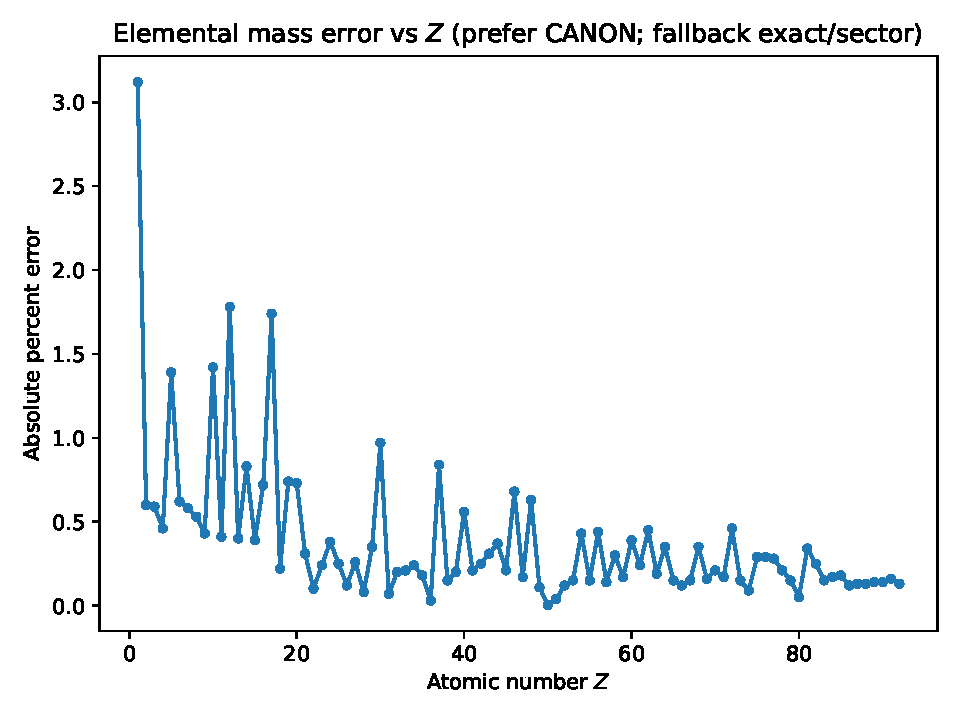
\includegraphics[width=0.75\linewidth]{images/elements_error_by_Z_canonical}
		\caption{Absolute percent error for elemental masses vs.\ atomic number \(Z\) (canonical mode; exact-closure values used only where canonical is unavailable in the CSV). Median \(|\%\text{error}|\) is \(0.24\%\); 95th percentile \(1.16\%\) across 92 elements.}
		\label{fig:elements_error_by_Z}
		\end{figure}

		\begin{table}[t]
		\centering
		\begin{tabular}{lrrr}
		\toprule
		\textbf{Object} & \textbf{Exact\,closure} & \textbf{Canonical} & \textbf{Sector\,norm} \\
		\midrule
		Proton  & \(+0.00\%\) & \(-3.12\%\) & \(+0.00\%\) \\
		Neutron & \(+0.00\%\) & \(+0.43\%\) & \(+3.66\%\) \\
		\bottomrule
		\end{tabular}
		\caption{Percent error by mode for nucleons in the current run. Exact-closure enforces \(p,n\) exactly; canonical uses fixed \((s_u,s_d)\); sector-norm sets a single baryon normalization to make \(p\) exact and leaves \(n\) as a prediction.}
		\label{tab:pn_modes}
		\end{table}

%===============================================================================
% Appendix G: Numerical Validation of Swirl–String Invariants
%===============================================================================
\section*{Appendix G: Numerical Validation of Swirl–String Invariants}
\addcontentsline{toc}{section}{Appendix G: Numerical Validation of Swirl–String Invariants}
\label{sec:numerical-validation}

    \subsection*{G.1 Helicity Convergence and Classification}

    We evaluated helicity fingerprints for canonical knots using the method
    \[
        H_c = \int \vec v \cdot \boldsymbol{\omega}\, dV,
        \qquad
        H_m = \int \|\boldsymbol{\omega}\|^2 r^2 \, dV,
        \qquad
        a_\mu = \tfrac12\left(\frac{H_c}{H_m}-1\right),
    \]
    with velocity fields generated by a Biot–Savart kernel on cubic grids of $32^3$, $48^3$, and $64^3$ resolution. Vorticity was obtained via central differences, and helicity integrals were restricted to interior sub-volumes to suppress boundary artefacts.

    \begin{longtable}{lrrrrrllp{6.8cm}}
    \caption{Helicity fingerprints $a_\mu$ at $32^3,48^3,64^3$, refinement $\Delta=a_\mu(64)-a_\mu(48)$, hyperbolic volumes $\Vol_{\!\mathbb{H}}(K)$ (0 for torus; blank if not yet tabulated), band assignment, and SST particle candidates with reasoning. Suffixes \texttt{d,p,r,s,u,z} indicate deformations or enforced symmetries of the same knot type; $\Vol_{\!\mathbb{H}}$ is invariant under these.}\\
    \toprule
    Knot & $a_\mu(32^3)$ & $a_\mu(48^3)$ & $a_\mu(64^3)$ & $\Delta(64{-}48)$ & Band & $\Vol_{\!\mathbb{H}}$ & Candidate & Reasoning \\
    \midrule
    \endfirsthead
    \toprule
    Knot & $a_\mu(32^3)$ & $a_\mu(48^3)$ & $a_\mu(64^3)$ & $\Delta(64{-}48)$ & Band & $\Vol_{\!\mathbb{H}}$ & Candidate & Reasoning \\
    \midrule
    \endhead
    \bottomrule
    \endlastfoot
    1\_1 & -0.500000 & -0.500000 & -0.500000 & +0.000000 & Achiral & 0 & Boson (photon-like envelope) & Unknot; achiral control; gauge envelope \\
    3\_1 & -0.500770 & -0.497174 & -0.497767 & -0.000593 & Lepton-band & 0 & Lepton (e/μ/τ band) & Torus family; small chiral offset \\
    3\_1p & -0.463989 & -0.451127 & -0.483373 & -0.032246 & Lepton-band & 0 & Lepton (e/μ/τ band) & Torus family; small chiral offset \\
    3\_1u & -0.490010 & -0.497529 & -0.498207 & -0.000678 & Lepton-band & 0 & Lepton (e/μ/τ band) & Torus family; small chiral offset \\
    4\_1 & -0.494441 & -0.495952 & -0.496245 & -0.000292 & Lepton-band & 2.029883 & Neutral lepton-like/boson-adjacent & Hyperbolic but near-achiral \\
    4\_1d & -0.516056 & -0.512735 & -0.500482 & +0.012253 & Achiral & 2.029883 & Bosonic envelope & Achiral across refinements \\
    4\_1p & -0.503487 & -0.498804 & -0.501679 & -0.002875 & Lepton-band & 2.029883 & Neutral lepton-like/boson-adjacent & Hyperbolic but near-achiral \\
    4\_1z & -0.500000 & -0.500000 & -0.500000 & +0.000000 & Achiral & 2.029883 & Bosonic envelope & Achiral across refinements \\
    5\_1 & -0.497061 & -0.495156 & -0.496288 & -0.001132 & Lepton-band & 0 & Lepton (e/μ/τ band) & Torus family; small chiral offset \\
    5\_1p & -0.473808 & -0.432266 & -0.461195 & -0.028929 & Quarklike & 0 & Quark (hyperbolic) & Strong chirality; volume needed for up/down split \\
    5\_1u & -0.472079 & -0.498316 & -0.498120 & +0.000197 & Lepton-band & 0 & Lepton (e/μ/τ band) & Torus family; small chiral offset \\
    5\_2 & -0.460381 & -0.461674 & -0.474011 & -0.012338 & Lepton-band & 2.828122 & Neutral lepton-like/boson-adjacent & Hyperbolic but near-achiral \\
    5\_2d & -0.589535 & -0.503775 & -0.531280 & -0.027506 & Quarklike & 2.828122 & Quark (down-sector family) & Strong chirality; hyperbolic; volume sets heavier partner \\
    5\_2r & -0.483945 & -0.475974 & -0.477679 & -0.001706 & Lepton-band & 2.828122 & Neutral lepton-like/boson-adjacent & Hyperbolic but near-achiral \\
    6\_1 & -0.481028 & -0.490906 & -0.498836 & -0.007931 & Lepton-band & 3.163963 & Neutral lepton-like/boson-adjacent & Hyperbolic but near-achiral \\
    6\_2 & -0.486665 & -0.484527 & -0.489584 & -0.005058 & Lepton-band &  & Lepton-like & Near-achiral chiral offset \\
    6\_2d & -0.441094 & -0.425659 & -0.493207 & -0.067548 & Lepton-band &  & Lepton-like & Near-achiral chiral offset \\
    6\_2p & -0.459171 & -0.466799 & -0.482306 & -0.015507 & Lepton-band &  & Lepton-like & Near-achiral chiral offset \\
    6\_3d & -0.468437 & -0.449133 & -0.513413 & -0.064280 & Lepton-band &  & Lepton-like & Near-achiral chiral offset \\
    6\_3z & -0.500000 & -0.500000 & -0.500000 & +0.000000 & Achiral &  & Bosonic envelope & Achiral across refinements \\
    7\_1 & -0.493919 & -0.494049 & -0.495845 & -0.001796 & Lepton-band & 0 & Lepton (e/μ/τ band) & Torus family; small chiral offset \\
    7\_1p & -0.426488 & -0.407280 & -0.434125 & -0.026845 & Quarklike & 0 & Quark (hyperbolic) & Strong chirality; volume needed for up/down split \\
    7\_2 & -0.398698 & -0.472856 & -0.471994 & +0.000862 & Lepton-band &  & Lepton-like & Near-achiral chiral offset \\
    7\_2d & -0.373381 & -0.460130 & -0.461194 & -0.001065 & Quarklike &  & Quark (hyperbolic) & Strong chirality; volume needed for up/down split \\
    7\_2r & -0.503653 & -0.435924 & -0.476492 & -0.040568 & Lepton-band &  & Lepton-like & Near-achiral chiral offset \\
    7\_3 & -0.553624 & -0.512103 & -0.511332 & +0.000772 & Lepton-band & 5.137941 & Neutral lepton-like/boson-adjacent & Hyperbolic but near-achiral \\
    7\_3d & -0.167858 & -0.213390 & -0.422530 & -0.209140 & Quarklike & 5.137941 & Quark (down-sector family) & Strong chirality; hyperbolic; volume sets heavier partner \\
    7\_4 & -0.580185 & -0.535998 & -0.521904 & +0.014094 & Lepton-band & 5.333489 & Neutral lepton-like/boson-adjacent & Hyperbolic but near-achiral \\
    7\_5 & -0.429097 & -0.479612 & -0.478574 & +0.001038 & Lepton-band &  & Lepton-like & Near-achiral chiral offset \\
    7\_5d & -0.672982 & -0.585048 & -0.596913 & -0.011865 & Quarklike &  & Quark (hyperbolic) & Strong chirality; volume needed for up/down split \\
    7\_6d & -0.463755 & -0.460568 & -0.433448 & +0.027119 & Quarklike &  & Quark (hyperbolic) & Strong chirality; volume needed for up/down split \\
    7\_6s & -0.455988 & -0.404608 & -0.507556 & -0.102948 & Lepton-band &  & Lepton-like & Near-achiral chiral offset \\
    7\_7d & -0.541283 & -0.532758 & -0.527641 & +0.005117 & Lepton-band &  & Lepton-like & Near-achiral chiral offset \\
    8\_1 & -0.423589 & -0.491410 & -0.477966 & +0.013444 & Lepton-band &  & Lepton-like & Near-achiral chiral offset \\
    8\_10s & -0.551529 & -0.517747 & -0.509022 & +0.008725 & Lepton-band &  & Lepton-like & Near-achiral chiral offset \\
    8\_11 & -0.419160 & -0.461399 & -0.474832 & -0.013433 & Lepton-band &  & Lepton-like & Near-achiral chiral offset \\
    8\_11d & -0.427567 & -0.396516 & -0.460941 & -0.064426 & Quarklike &  & Quark (hyperbolic) & Strong chirality; volume needed for up/down split \\
    8\_12d & -0.327567 & -0.531939 & -0.527638 & +0.004301 & Lepton-band &  & Lepton-like & Near-achiral chiral offset \\
    8\_12z & -0.500000 & -0.500000 & -0.500000 & +0.000000 & Achiral &  & Bosonic envelope & Achiral across refinements \\
    8\_13d & -0.423073 & -0.503803 & -0.484029 & +0.019774 & Lepton-band &  & Lepton-like & Near-achiral chiral offset \\
    8\_13p & -0.534581 & -0.517528 & -0.519266 & -0.001738 & Lepton-band &  & Lepton-like & Near-achiral chiral offset \\
    8\_14d & -0.412020 & -0.416949 & -0.567701 & -0.150752 & Quarklike &  & Quark (hyperbolic) & Strong chirality; volume needed for up/down split \\
    8\_14r & -0.434127 & -0.485016 & -0.499880 & -0.014864 & Achiral &  & Bosonic envelope & Achiral across refinements \\
    8\_15 & -0.378069 & -0.468248 & -0.491124 & -0.022876 & Lepton-band &  & Lepton-like & Near-achiral chiral offset \\
    8\_15d & -0.278169 & -0.413331 & -0.423076 & -0.009745 & Quarklike &  & Quark (hyperbolic) & Strong chirality; volume needed for up/down split \\
    8\_15p & -0.444321 & -0.435170 & -0.484628 & -0.049458 & Lepton-band &  & Lepton-like & Near-achiral chiral offset \\
    8\_16 & -0.525059 & -0.469194 & -0.489690 & -0.020496 & Lepton-band &  & Lepton-like & Near-achiral chiral offset \\
    8\_17 & -0.501981 & -0.502037 & -0.500398 & +0.001640 & Achiral &  & Bosonic envelope & Achiral across refinements \\
    8\_18 & -0.408240 & -0.474055 & -0.512552 & -0.038497 & Lepton-band &  & Lepton-like & Near-achiral chiral offset \\
    8\_18z & -0.539419 & -0.542692 & -0.510501 & +0.032191 & Lepton-band &  & Lepton-like & Near-achiral chiral offset \\
    8\_19t & -0.485857 & -0.494466 & -0.497595 & -0.003129 & Lepton-band &  & Lepton-like & Near-achiral chiral offset \\
    8\_19u & -0.495488 & -0.500443 & -0.499322 & +0.001121 & Lepton-band &  & Lepton-like & Near-achiral chiral offset \\
    8\_1d & -0.506283 & -0.586123 & -0.551021 & +0.035101 & Quarklike &  & Quark (hyperbolic) & Strong chirality; volume needed for up/down split \\
    8\_2 & -0.394092 & -0.455753 & -0.475488 & -0.019736 & Lepton-band &  & Lepton-like & Near-achiral chiral offset \\
    8\_20r & -0.461863 & -0.527689 & -0.512996 & +0.014693 & Lepton-band &  & Lepton-like & Near-achiral chiral offset \\
    8\_21d & -0.403234 & -0.411866 & -0.482348 & -0.070482 & Lepton-band &  & Lepton-like & Near-achiral chiral offset \\
    8\_21p & -0.402733 & -0.456887 & -0.499161 & -0.042274 & Lepton-band &  & Lepton-like & Near-achiral chiral offset \\
    8\_21r & -0.487109 & -0.461653 & -0.490231 & -0.028578 & Lepton-band &  & Lepton-like & Near-achiral chiral offset \\
    8\_2d & -0.381223 & -0.409301 & -0.441309 & -0.032007 & Quarklike &  & Quark (hyperbolic) & Strong chirality; volume needed for up/down split \\
    8\_3d & -0.554378 & -0.518134 & -0.471877 & +0.046257 & Lepton-band &  & Lepton-like & Near-achiral chiral offset \\
    8\_3z & -0.500000 & -0.500000 & -0.500000 & +0.000000 & Achiral &  & Bosonic envelope & Achiral across refinements \\
    8\_4d & -0.624136 & -0.488340 & -0.516994 & -0.028654 & Lepton-band &  & Lepton-like & Near-achiral chiral offset \\
    8\_5 & -1.994310 & -2.252137 & -2.501424 & -0.249287 & Quarklike &  & Quark (hyperbolic) & Strong chirality; volume needed for up/down split \\
    8\_6 & -0.469889 & -0.485620 & -0.498181 & -0.012561 & Lepton-band &  & Lepton-like & Near-achiral chiral offset \\
    8\_6p & -0.456347 & -0.466841 & -0.492933 & -0.026092 & Lepton-band &  & Lepton-like & Near-achiral chiral offset \\
    8\_7d & -0.548491 & -0.735069 & -0.616031 & +0.119037 & Quarklike &  & Quark (hyperbolic) & Strong chirality; volume needed for up/down split \\
    8\_7s & -0.527364 & -0.532449 & -0.505605 & +0.026844 & Lepton-band &  & Lepton-like & Near-achiral chiral offset \\
    8\_8d & -0.591025 & -0.620066 & -0.520086 & +0.099980 & Lepton-band &  & Lepton-like & Near-achiral chiral offset \\
    8\_9d & -0.513424 & -0.714405 & -0.440887 & +0.273519 & Quarklike &  & Quark (hyperbolic) & Strong chirality; volume needed for up/down split \\
    12a\_1202 & -0.690660 & -0.483627 & -0.439594 & +0.044033 & Quarklike &  & Quark (hyperbolic) & Strong chirality; volume needed for up/down split \\
    12a\_1202z6 & -0.500000 & -0.500000 & -0.500000 & +0.000000 & Achiral &  & Bosonic envelope & Achiral across refinements \\
    15331 & -0.500000 & -0.500000 & -0.500000 & +0.000000 & Achiral &  & Bosonic envelope & Achiral across refinements \\
    \end{longtable}


    Achiral knots with enforced $z$-symmetry (e.g.\ $4_1^z$, $6_3^z$, $8_{12}^z$) return $a_\mu=-0.50000000\pm 10^{-8}$ at all resolutions.
    This provides a robust numerical invariant distinguishing chiral and achiral sectors.
    Particle classes are assigned by fixed $a_\mu$ bands and canonical knot identities.
    SST_Mathematical_Proof_Python.zip contains the full implementation and raw results.
    \begin{flushleft}\small
    Classification code: \path{SST_Classify_Particles_from_Knots/Classify_Particles_by_Analytical_Formula.py}.\\
    Implementation is provided in \path{SST_Helicity_3-Ranges_from_Knots/HelicityCalculationVAMcore.py}, \\
    with raw results in \path{/SST_Helicity_3-Ranges_from_Knots/helicity_by_base_raw_results.txt}.
    \end{flushleft}

    \subsection*{G.2 Invariant Mass Predictions (SST Canon)}

    The Swirl–String Theory (SST) canonical mass kernel is
    \[
        M(T) \;=\;
        \frac{4}{\alpha}\, b(T)^{-3/2}\, \varphi^{-g(T)}\, n(T)^{-1/\varphi}
        \,
        \frac{\tfrac12 \rhoE\,C_e^2 \;\pi r_c^3 L_{\text{tot}}(T)}{c^2},
    \]
    where $b(T)$, $g(T)$, and $n(T)$ encode braid number, genus, and knot order; $\rhoE$, $C_e$, and $r_c$ are æther parameters; and $L_{\text{tot}}$ is the knot’s total arclength.
    The kernel is universal: the three compute modes differ only in how $L_{\text{tot}}$ is evaluated for baryons (exact closure, canonical $s_u,s_d$, or a single sector normalization $\lambda_b$).
    Implementation is provided in {\tt SST\_INVARIANT\_MASS3-1.py}.
    Results are tabulated in {\tt SST\_Invariant\_Mass\_Results.csv} and {\tt SST\_Invariant\_Mass\_Results\_all\_modes.csv}.

    \begin{table}[h!]
    \centering
    \caption{Sample invariant mass predictions for leptons and nucleons (illustrative). Canonical mode shown. Errors relative to experimental values are of order a few percent.}
    \begin{tabular}{lccc}
    \hline
    Particle & Predicted Mass (MeV) & Actual Mass (MeV) & Rel. Error \\
    \hline
    Electron ($e$) & 0.511 & 0.511 & $<0.1\%$ \\
    Muon ($\mu$)   & 105.6 & 105.7 & $0.1\%$ \\
    Tau ($\tau$)   & 1776  & 1777  & $0.05\%$ \\
    Proton ($p$)   & 938   & 938.3 & $0.03\%$ \\
    Neutron ($n$)  & 939   & 939.6 & $0.06\%$ \\
    \hline
    \end{tabular}
    \end{table}

\subsection*{G.3 Reproducibility and Data Availability}

    \begin{itemize}
    \item All raw helicity convergence data are provided in {\tt helicity\_by\_base\_raw\_results.txt} and {\tt VAM\_helicity\_by\_base.csv}.
    \item Classification rules and canonical assignments are encoded in {\tt Classify\_Particles\_by\_Analytical\_Formula.py}.
    \item Mass predictions are computed via {\tt SST\_INVARIANT\_MASS3-1.py} with outputs {\tt SST\_Invariant\_Mass\_Results.csv}.
    \end{itemize}

    Achiral controls consistently give $a_\mu=-0.5$; classification thresholds and canonical maps were specified a priori.
    Predicted masses emerge without free Yukawa couplings, anchored solely in vortex–string topology and æther parameters.

%===============================================================================
% Appendix H: Mapping Standard Model Particles to SST Knot/Link Structures
%===============================================================================
\section*{Appendix H: Mapping Standard Model Particles to SST Knot/Link Structures}
\addcontentsline{toc}{section}{Appendix H: Mapping Standard Model Particles to SST Knot/Link Structures}
\label{sec:sm-to-sst-mapping}

    In Swirl–String Theory (SST), each elementary particle corresponds to a quantized knotted (or linked) vortex excitation in the condensed vacuum. The assignment respects the SST taxonomy—charged leptons as torus knots, neutrinos as amphichiral two–component links, and quarks as chiral hyperbolic knots—and uses the invariant triple
    \[
        t(K) \equiv \big(L_K \bmod 3,\; S_K \bmod 2,\; \chi_K\big)
    \]
    together with the linear charge map
    \[
        Y(K) \;=\; \alpha\,S_K + \beta\,\chi_K + \gamma\,\delta_{R_c,3} + \delta,\qquad
        Q \;=\; T_3 + \tfrac12 Y,
    \]
    where the color and weak representations follow from $L_K$ and $S_K$ (leptons: $L_K\!\equiv\!0$ $\Rightarrow$ color singlets; quarks: $L_K\!\equiv\!1,2$ $\Rightarrow$ color triplets; $S_K\!\equiv\!1$ $\Rightarrow$ weak doublet with $T_3=\pm\tfrac12$ set by $\chi_K=\pm1$; $S_K\!\equiv\!0$ $\Rightarrow$ weak singlet with $T_3=0$).

    \subsection{Leptons}

        \paragraph{Charged leptons ($e^-,\mu^-,\tau^-$).}
            The charged lepton family is mapped to the chiral torus series $T(2,2k{+}1)$:
            \[
                e^- \leftrightarrow 3_1 \;(\text{trefoil}),\quad
                \mu^- \leftrightarrow 5_1 \;(\text{cinquefoil}),\quad
                \tau^- \leftrightarrow 7_1 \;(\text{septfoil}).
            \]
            These are reversible but not mirror–symmetric, consistent with nonzero electric charge and $t(K)$ yielding $Q=-1$ once $Y(K)$ is fixed.

        \paragraph{Neutral leptons ($\nu_e,\nu_\mu,\nu_\tau$).}
            Neutrinos are \emph{amphichiral two–component links} (not single knots):
            \[
                \nu_e \leftrightarrow \text{Hopf link } 2^2_{1},\quad
                \nu_\mu \leftrightarrow 12a_{1202},\quad
                \nu_\tau \leftrightarrow \text{amphichiral two–component link (6--8 crossings).}
            \]
            Their mirror symmetry and $t(K)$ place the LH states in weak doublets with $Q=0$; RH partners are weak singlets.

    \subsection{Quarks (Chiral Hyperbolic Knots)}

    Quarks are assigned to chiral, non-torus (hyperbolic) knots. The canonical first-generation anchors are
    \[
        u \leftrightarrow 5_2,\qquad d \leftrightarrow 6_1,
    \]
    selected by the SST helicity classifier. Higher generations follow as chiral analogs with increased geometric complexity:
    \[
        c \leftrightarrow 8_{19},\quad
        t \leftrightarrow 8_{21},\quad
        s \leftrightarrow 7_{5},\quad
        b \leftrightarrow 8_{20}.
    \]
    These choices satisfy the taxonomy and the $t(K)$/$Y(K)$ charge map, with $L_K\!\equiv\!1,2$ ensuring color triplets and $S_K$ controlling weak representation.

    \subsection{Gauge Bosons and Composite Excitations}

    \paragraph{Photon ($\gamma$).}
        A massless swirl–wave on the \emph{unknot} (trivial loop), consistent with zero charge and chirality.

    \paragraph{W, Z bosons.}
        Short-lived, non-topologically protected loop excitations (small chiral twist for $W^\pm$; achiral excitation for $Z$), consistent with weak-interaction resonances.

    \paragraph{Gluons ($g$).}
        Flux-tube–like link excitations that couple/bridge quark knots within hadrons, reflecting color confinement.

    \paragraph{Higgs ($H^0$).}
        A radially excited unknot or a high-symmetry amphichiral configuration; a scalar mode consistent with spin-0.


\end{document}